
%//////////////////////////////////////////////////////////////////////
% 2022年度 情報学群実験第3i・第4C テキスト
%                                       高知工科大学情報学群
%//////////////////////////////////////////////////////////////////////
\documentclass[10pt]{text2002}
\usepackage{eclbkbox}
\usepackage{alltt}
\usepackage{ascmac}
\usepackage[dvipdfmx]{graphicx}
\usepackage{graphicx}
\usepackage{multicol}
\usepackage{fancybox}
\usepackage{jumoline}
\usepackage{url}

%\usepackage[nobottomtitles]{titlesec}
%\widowpenalty10000
%\clubpenalty10000

\newcommand{\ttt}[1]{\texttt{#1}}

% \makeatletter
%      \def\sloppy{%
%        \tolerance 9999%
%        \emergencystretch 3em%
%        \hfuzz .5\p@
%        \vfuzz\hfuzz}
% \makeatother

%	enumerate 環境の変更
\renewcommand{\labelenumi}{(\theenumi)}

%	keybox(ascmac.sty の \keytop の中身をタイプライタ体に変更)
\def\keybox#1{{\keytop{\tt#1}}}

%	taskbar(文字列を囲む枠)
\def\taskbar#1{\setlength{\fboxrule}{0.5pt}\fbox{#1}}

%	Hline(tabular 環境内の \hline よりも太い横線)
%		from IEICE LaTeX Macro
\def\Hline{\noalign{\hrule height 0.4mm}}
%	enumerate 環境の変更
\renewcommand{\labelenumi}{(\theenumi)}

%	Gcenter(tabular 環境内の縦方向のセンタリング)
%		written by Otobe Yoshiki
\newcommand{\Gcenter}[2]{
    \dimen0 = \ht\strutbox
    \advance\dimen0\dp\strutbox
    \multiply\dimen0 by#1
    \divide\dimen0 by2
    \advance\dimen0 by-.5\normalbaselineskip
    \raisebox{-\dimen0}[0pt][0pt]{#2}}

  \makeatletter
    \newenvironment{cli}%
    {\VerbatimEnvironment
     \begin{center}
     \begin{breakbox}
     \begin{Verbatim}
        }%
    {%
     \end{Verbatim}
     \end{breakbox}
     \end{center}
     }
  \makeatother

  \makeatletter
    \newenvironment{cli-tex}%
    {\begin{center}
     \begin{breakbox}
     \begin{alltt}
        }%
    {%
     \end{alltt}
     \end{breakbox}
     \end{center}
     }
  \makeatother

\newif\ifTA
\TAfalse

\title{}
\author{}
\date{}

\begin{document}
\sloppy
\maketitle
%----------------------------------------------------------------------- 目次
\pagenumbering{roman}
%   目次はローマ数字
\chapter*{序~~論}\label{chapter:introduction}
%
%   はじめに
%        written by Shinichi Yoshida
%        April 13, 2018

昨今,人工知能(機械学習とビッグデータ処理)関連の技術の進展が目覚しく,
人間の行う職業がなくなりつつあるように見受けられる.例えば,自動運転技術
が進展することで,バスやトラック,タクシーなどの職業が衰退することも考え
られる.エンジニア職も例外ではない.ネットワークエンジニアは将来なくなる
職業にとりあげられることもある.しかしながら,人工知能技術は,明確なルー
ルがあるものや,単調な作業などはすぐに置き換えることができるが,複雑なも
のになればなるほど,機械学習アルゴリズムでは学習ができない.一方,ネット
ワーク技術が様々な技術の集合体であり,場所によって異なる形で構築がされる
ような複雑なシステムである.全ての機器が設計通りに動いているのならばまだ
しも,停電や経年劣化,障害等で一部の機器が動作停止や誤動作するようなこと
もある.こうした複雑かつ困難な状況に,即座に柔軟に対処できるような AI は
まだ見当たらない.このような観点から考えると,ますます複雑になるネットワー
クシステムを支える技術者は,今後しばらくは(少なくとも我々が職業を持って
働く間は)なくなることはないであろう.

さらに言えば,Facebook, Twitter, LINE などの SNS,Google, Dropbox,
Amazon, Microsoft 等の様々なサービスやクラウド技術など,インターネットサー
ビスが発展し,多くの人々が利用している.これらは,インターネットのインフ
ラが稼働していないと全く利用できない.すなわち,これらに障害が起きると生
活に支障が出るくらい,重要な生活のインフラストラクチャ(基盤)になってい
ると言え,これらを支えることは現代では電気・エネルギーや水道,運輸インフ
ラを支えると同じくらい重要なことである.

また,セキュリティも重要な事項であり,他のインフラと異なり,インターネッ
トインフラはサイバー攻撃による影響がとても大きく,一つの企業や国の生活に
影響を与えるほどである.実際に,通常の軍隊と同様に,サイバー軍を創設し他
国への攻撃,他国からの攻撃に備える国も増えている.さらには,先ほどの人工
知能も人々のインターネットの利用が進み,さらには IoT (Internet of
Things) などで多くの機器がインターネット接続され,多くのデータが蓄積され
たことで,はじめて人工知能が構築可能になったとも言える.

以上のことから,インターネット技術を実際に体験し習得することは,今後の情
報技術者にとって重要なことであるのは間違いない.この実験では,こうしたイ
ンターネット技術を支える技術について,実際に構築をしながら,幅広い角度か
らネットワーク技術を学ぶ.本実験で扱う技術は,必ずしも最新のサービスでは
なく,今後も長く使われ続ける基礎技術に重点を置いている.UNIX系OS(Ubuntu
Linux,CentOS), Windows, Macintosh といった広く普及しているオペレーティ
ングシステムを用いて,それぞれのコンピュータのネットワーク設定ならびに,
サーバでのWWWやデータベースシステム,暗号化など,身近に使われているネッ
トワークサービスの構築を行う.さらに,ルーティング,ネットワーク設計,ス
イッチ設定,VLAN,セキュリティといったインターネットを支える基盤技術の構
築を,ネットワーク業界で広く使われる Cisco IOS を実際に用いて学ぶ.IOS 
は CCNA 試験など,ネットワーク業界で認められている資格試験にも使われてお
り,多くのベンダが IOS 互換のコマンド体系を採用していることからネットワー
クを学ぶのに最も適したシステムといっても良い.

本実験の内容は初学の者にとっては十分に複雑で難しいものであるかも知れな
い.しかし,本実験の内容はまだまだ基礎であり,この先にはさらに複雑で設
計の難易度の高いシステムが数多く存在している.ぜひ,この実験を通して基
礎技術,基盤技術を身に付け,将来,更なる発展技術の習得,および新技術,
新サービスの開発へと進んでいき,インターネットの発展に寄与して欲しいと
考える.

全ての専攻の学生が,このテキストと実験での経験をもとに,ネットワーク技術
の仕組みを理解し,様々な業界で活躍することを心より期待し,巻頭の言とする.

\begin{flushright}
 2019年4月13日

 情報学群実験3i・4C 教育担当スタッフ一同
\end{flushright}

\clearpage
\chapter*{レポートについて}\label{chapter:report}


レポートは,下記の体裁にて提出すること.\textbf{全てのレポートについて,
1つでも下記に該当する場合,採点および単位認定されない} ので注意すること.

\begin{itemize}
 \item \textbf{指定された期日・時刻までに提出されない場合}
 \item \textbf{指定された様式でない場合,特に抜けている項目がある場合}
\end{itemize}

加えて,\textbf{下記の場合は,単位認定されない上に,不正行為として処罰さ
れる行為}であるので,厳に慎むこと.

\begin{itemize}
 \item \textbf{他人のレポートからの転載}
 \item \textbf{他の Web ページ,本などからの転載}
\end{itemize}

本科目のレポートは,全て,KUT LMS (Learning Management System,
https://lms.kochi-tech.ac.jp )の本科目の項目から PDF にて提出する.提出
されたレポートは,\textbf{Turnitin システムにより,過去も含む他人のレポー
ト,Webページ,出版された本などと一致する文章があるか照合され,剽窃チェッ
クが行われる.}

LaTeX (platex) にて,実験の冒頭で指定されたテンプレートを用いて作成する
こと.

\textbf{章立ては下記の通りとすること.下記の項目に従っていないもの,一部の項目に
抜けがある不完全なものは,提出されても受理しない.}

\begin{description}
 \item[1. 目的] それぞれの回で,どのようなことができるシステムを構築する
	    のかと,なぜそのシステムが必要であるか,構築することでどのよ
	    うな機能・サービスが実現できるのかを述べる.ただし,自らの学
	    習目的,学ぶ内容を説明しないように注意する(○○を習得する,
	    学ぶ,などと書かない)(2点満点).
 \item[2. 内容] 構築するシステムの技術的な説明(どのような要素技術を用い
	    て,どのような仕組み・原理で実現するのか)を,システムの全体
	    像が分かるような\textbf{説明図を1つ以上含めて説明する}.図を用いて,
	    実際の挙動の例などを説明する(2点満点).
 \item[3. 要素技術] システムで用いられる要素技術について,指定されたもの
	    について,それがどのようなものであるか,技術的背景,仕組み,
	    構造,動作について説明する.ただし,あくまで技術の解説をし,
	    単なる用語説明にならないように注意する.また,適切な参考文献
	    を挙げて根拠を示すこと(2点満点).
 \item[4. 作業記録] システムを構築するために,具体的にどのような作業をし
	    たかを記録する.用いたソフトウェア,行った操作,コマンド,設
	    定した内容,編集したファイルなどをもれなく書く.システムが壊
	    れた場合など,一から構築するときも,記述された作業を行うこと
	    で,全く同じシステムを構築することができるように書く(2 点満
	    点).
 \item[5. 考察] 考察のポイントを踏まえて,取り扱うシステム・技術の利点や
	    欠点,その技術の本質,類似システムとの相違・相似などの比較・
	    考察を行い,自分なりの考え,結論を書く(結論は感想ではない.
	    ○○という技術は▽▽の一種であるから本質的にこのような問題を
	    抱えている.ゆえに,将来□□を改良・解決した◇◇などの研究・
	    開発が重要である,など)(2点満点).
 \item[参考文献] 第1節から第5節までで述べたことのうち,自ら考案したオリ
	    ジナルの意見でなければ(あるいは考案したことであっても,過去
	    同じことが発明・提案されているならば),その内容について述べ
	    ている文献を適切に挙げること.記述の例として,下記のように書
	    くこと.\textbf{最低5つ程度の参考文献は挙げること.また,一
	    般のWebページの引用は原則できない.文中で適切に引用すること.
	    参考文献がほとんどないものは項目抜けとして扱う.}

	    \begin{itemize}
	     \item 本を参考にする例\\

	    (例) 佐伯サチオ,福冨エイジ著,福本昌弘監修,吉田真一訳:
	    「情報実験の方法論」,pp. ○〜○ (どのぺージに書いてあるか),
	    KUT出版,2012(発行年).

	     \item 雑誌を参考にする例\\

	    (例) 吉田真一:「情報実験の方法論(記事名)」,○○雑誌名,
	    ○巻,○号,pp. ○〜○ (ぺージ to ページ),KUT出版,2012 
	    (発行年).

	     \item 英文等の例\\

	    (例) Shinichi Yoshida, Sachio Saiki, and Eiji Fukutomi, ``
		   Computer Network,'' Journal of KUT, Vol. 3, No. 4,
		   pp. 501-511, 2012.\\

		   2種類のダブルクォーテーション,始まり「``」(LaTeXでは,
		   バッククォーテーション \verb|`| を2つタイプ \verb|`| \verb|`|) と,
		   終わり '' (LaTeXでは,シングルクォーテーション
		   \verb|'| を2つタイプ \verb|'| \verb|'|)に注意し,項
		   目の区切りには半角コ
		   ンマ「,」を使い,コンマの後ろには必ず半角空白を1つタ
		   イプする.終わりのダブルクォーテーションの後に項目を
		   続ける場合は,コンマはダブルクォーテーションの前に入
		   れ,最後は半角ピリオド「.」で終わる.


	    \end{itemize}

 \item[(付録や感想)] その他,気がついたことで報告しておきたいことを付
	    録として報告しても良い.また感想を付けても構わない.ただし,
	    節番号を付けないこと.ただし,「付録」「感想」とも直接的には
	    採点の対象とはならない.また,「付録」「感想」に書かれた内容
	    は,レポートの採点には(良い方にも悪い方にも)影響しない.

\end{description}

忘れがちな点を下記に示す.
\begin{itemize}
 \item {\bf 日本語文の場合,コンマ「.」やピリオド「.」は全角を
		   用いる.}
 \item {\bf 英文の場合,コンマ「,」やピリオド「.」は半角を用い,コン
       マの後に半角空白を1つ,ピリオドの後に半角空白を2つタイプする.}
 \item 意味的に1つのトピックごとに段落分け(パラグラフ)し,パラ
       グラフの区切りには,\LaTeX の場合,{\bf 空行を1行}入れると,自動的に次
       段落1行目を1文字インデントするので,これを用いる.{\bf 強制改
       行「\verb|\|\verb|\|」あるいは「\bf \yen\yen」は段落分けには用いず},段落の1行目の最初にも全角空
       白「 」は挿入しない.
\end{itemize}


分量は特に指定しないが,目的,内容,考察の各項目を十分に説明するには,そ
れぞれ,数百字程度は必要であると期待される.また,要素技術について
も,それぞれの技術項目について数百字程度は期待される.

\textbf{著作権 (Copyright)} やその他の知的財産権(Intellectual Property),
の処理については,十分に注意をすること.具体的には,著作者の許可を得ずに
本・教科書・Webページ等の記述・図・表の転載などを行わないようにすること.

また,\textbf{倫理上の問題やコンプライアンス(法令,政令等の法律や国の規定,通達,学則
や「高知工科大学における研究活動の不正行為への対応等に関する規程」等の学
内規則,判例等の司法判断,一般的な常識(社会通念上の規範)の遵守)} につ
いても十分留意すること.具体的には,不正と認定されるような行為(例えば他
人のレポート,文書,本,雑誌,Webからの転載)などを行わないこと.

最初にも述べたが,\textbf{他の文書(インターネット上の情報や他人のレポー
ト等)から文書の転載は,上記に違反するものであり,Q末試験におけるカンニ
ング等の不正行為と同様のものとして扱う.}



%  目次を出力
 \tableofcontents
\clearpage
%----------------------------------------------------------------------- 本文
%   本文のページ番号はアラビア数字
\pagenumbering{arabic}


%===================================================================== 第一部
\part{情報学群実験第3i・第4C}\label{part:1}

\chapter[オペレーティングシステムの導入とネットワーク設定]
{オペレーティングシステムの\\導入とネットワーク設定}\label{ch:os}
\def\chapos{01_1_os/}
\input{\chapos os.tex}
\def\chapnet{01_1_os/}
\input{\chapnet 02main.tex}

\chapter{DNS・メールサービス}\label{ch:dns}
\def\chapdns{01_2_dns_mail/}
\input{\chapdns 05main.tex}
\def\chapmail{01_2_dns_mail/}
\input{\chapmail 07main.tex}

\chapter{WWW システムと認証および暗号化}
\def\chapwww{02_1_http_auth_crypt/}
\input{\chapwww 04main.tex}

\chapter{データベース・Web システム}
\def\chapdb{02_2_database_websystem/}
\input{\chapdb 05main.tex}

\chapter{ルータ・スイッチ}\label{ch:patch}
\def\chaprouter{03_1_router_sw/}
\input{\chaprouter router.tex}
\def\chapsw{03_1_router_sw/}
\input{\chapsw switch.tex}

\chapter{ネットワークセキュリティ}
\def\chapfw{03_2_firewall/}
\input{\chapfw 06main.tex}

\chapter{最終課題}
\def\chapfinal{0Z_final/}
\input{\chapfinal 07main.tex}


%===================================================================== 第三部
\part{付~~録~~編}\label{part:appendix}
\appendix
\chapter{viエディタの使い方}\label{etc:vi}
%
%       「viエディタの使い方」
%               written by Masahiro Fukumoto
%               modified by Takahiko Mendori
%

\newcommand{\ckeywidth}{1.5zw}
\newcommand{\ckey}[1]{
 \framebox[\ckeywidth][c]{\texttt{#1}\phantom{Jj}\hspace*{-.85zw}}
}
\newcommand{\Esckey}{
 \framebox[2zw][c]{\textsf{Esc}\phantom{Jj}\hspace*{-.85zw}}
}
\newcommand{\Enterkey}{
 \framebox[3zw][c]{\textsf{Enter}\phantom{Jj}\hspace*{-.85zw}}
}


UNIXには Emacs や mule などの他に vi と呼ばれるエディタがある.
vi は UNIX で標準提供されているエディタで,
すべての UNIXシステム上で利用することができる
(Emacs は豊富な機能を持ったエディタであるが,
通常は標準で提供されてはいないため,
使用するためにはインストールする必要がある).

\section{vi の起動}

vi はファイル名を引数に与えて起動する
(ファイル名は省略できる).

\texttt{\% vi} [\textit{filename}]

\section{vi のモード}
vi には,コマンドモードと入力モードがある.
vi を起動した直後のモードはコマンドモードであり,文字を入力できる
モードにはなっていない.
コマンドモードでは,カーソルの移動,ファイルの保存,テキストの削除,
複写などの操作を行う.
文字を入力するには入力モードに入る必要がある.
コマンドモードから入力モードへの切替えは,\ckey{i}などのキーで,
また入力モードからコマンドモードへの切替えは\Esckey で行う.

\section{コマンドモード}
コマンドモードでは,コマンドに先行して数引数を与えることができ,
ほとんどのコマンドは数引数をコマンドの繰り返し数と解釈する.
例えば,\ckey{5}\ckey{j}と入力すれば 
\ckey{j}\ckey{j}\ckey{j}\ckey{j}\ckey{j}
と入力することと同じになる.

\subsection{カーソルの移動}
上下左右のカーソルの移動には,コマンドモードでそれぞれ
\ckey{k}\ckey{j}\ckey{h}\ckey{l}のキーを使う.
その他,カーソル移動のコマンド(キー)を以下にまとめる.
\\

\begin{center}
\begin{tabular}{c|l||c|l}
\hline
{\bf コマンド} & {\bf 移動先} & {\bf コマンド} & {\bf 移動先} \\ \hline
\texttt{j} & 1行下 & \texttt{G} & 最終行 \\
\texttt{k} & 1行上 & \textit{n}\texttt{G} & \textit{n}行目 \\
\texttt{h} & 1文字左 & \texttt{H} & 画面の最上行 \\
\texttt{l} & 1文字右 & \texttt{M} & 画面の中央行 \\
\texttt{0} & 現在行の先頭 & \texttt{L} & 画面の最下行 \\
\texttt{\$} & 現在行の行末 & \texttt{b, B} & 前の単語の先頭 \\
$\mathbf{\hat{\phantom{a}}}$ & 現在行の先頭の単語の先頭
 & \texttt{w, W} & 次の単語の先頭 \\
\framebox[3zw][c]{\textsf{Enter}} & 1行下の先頭 & \texttt{e, E}
 & 現在もしくは次の単語の末尾 \\
\hline
\end{tabular}
\end{center}

\subsection{削除,複写,移動}
テキストの削除には次のコマンドを使う.

\begin{center}
\begin{tabular}{c|l}
\hline
{\bf コマンド} & {\bf 意味} \\ \hline
\texttt{x} & カーソル位置の文字を削除 \\
\texttt{X} & カーソル位置の直前の文字を削除 \\
\texttt{dd} & 現在行を削除 \\
\texttt{dw} & カーソル位置からその単語の最後までを削除 \\
\texttt{d\$} & カーソル位置から行の最後までを削除 \\
\texttt{d}$\mathbf{\hat{\phantom{a}}}$ & カーソル位置から行の先頭までを削除 \\
\texttt{J} & 現在行と次行を 1行に連結 \\
\hline
\end{tabular}
\end{center}

vi は直前の削除あるいは置換コマンドによって消されたテキストを
退避バッファに保存している.
また,指定した領域を退避バッファに複写することもできる.
テキストを退避バッファに保存した後でカーソルを移動し,
退避バッファの内容を現在変集中のテキストに挿入することで,
テキストの移動や複写ができる.
以下にコマンドを示す.
\\

\texttt{
\begin{center}
\begin{tabular}{c|l}
\hline
{\bf コマンド} & {\bf 意味} \\ \hline
P & 退避バッファの内容をカーソル位置に挿入 \\
p & 退避バッファの内容をカーソル位置の直後に挿入 \\
yy & 現在行を退避バッファに保存 \\
yw & カーソル位置から単語の終りまでを退避バッファに保存 \\
\hline
\end{tabular} 
\end{center}
}

\subsection{検索,置換}
文字列の検索は,\ckey{/}の後に検索したい文字列を入力して 
\Enterkey キーを押す.
検索を繰り返す場合には,\ckey{n}を入力する.
また,前にさかのぼって検索する場合には\ckey{/}のかわりに 
\ckey{?}を用いる.

文字列を置換する場合は,まず\ckey{/}で文字列を検索し,
ここで\ckey{c}\ckey{w}の後に変更する文字列を入力して
\Esckey キーを押す.

\subsection{コマンドの取り消しと再実行}
vi では,直前の編集コマンドのみ取り消すことができる.
\ckey{u}を入力すると直前に実行されたコマンドが取り消される.
また,\ckey{.}は直前のコマンドを再実行する.

\subsection{ファイルの読み書き}
ファイルの読み書きはコマンドモードで行う.
作成(修正)したテキストをファイルとして書き込むためには 
\ckey{:}の後に\ckey{w}を入力する\footnote{
ただし,UNIXではファイルにオーナー,グループ,
パーミッション(使用許可)という属性があるため,
``\texttt{Read-only file, not written; use ! to override.}''
などのメッセージが表示され,書き込めないことがある
(書き込み不許可のパーミッションのとき).
パーミッションを変更する場合には \texttt{chmod}コマンド
({\bf 付録\ref{etc:unixcmd}} 参照)を用いる.}.

ファイルの読み書きや vi の終了などを行う場合には,通常 
\ckey{:}を入力する.
\ckey{:}を入力することにより最下行に`` : ''が表示されるから,
ここにコマンドを入力する.
ファイル操作のコマンド\footnote{
これらのコマンドは入力後に\Enterkey キーを押す必要がある.}
を以下に示す.
\\

\begin{center}
\begin{tabular}{l|l}
\hline
{\bf コマンド} & {\bf 機能} \\ \hline
\texttt{:w} & 現在のファイル名で保存 \\
\texttt{:w} \textit{filename} & \textit{filename}に保存 \\
\texttt{:w!} & 強制書き込み \\
\texttt{:e} \textit{filename} & \textit{filename}を新たに読み込み \\
\texttt{:e!} & ファイルの再読み込み \\
\texttt{:r} \textit{filename}
 & \textit{filename}の内容をカーソル行の次行に挿入 \\
\hline
\end{tabular}
\end{center}

\subsection{vi の終了}
vi の終了の方法には,ファイルに保存後終了,内容が更新されて
いる場合には警告メッセージを表示する終了,強制終了の 3通りがある.
それぞれの終了コマンドは次の通りである.
\\

\begin{center}
\begin{tabular}{l|l}
\hline
{\bf コマンド} & {\bf 機能} \\ \hline
\texttt{ZZ} & 編集中の内容を保存して vi を終了 \\
\texttt{:wq} [\textit{filename}] \framebox[3zw][c]{\textsf{Enter}}
 & 編集中の内容を \textit{filename} に保存し vi を終了 \\
\texttt{:q} \framebox[3zw][c]{\textsf{Enter}} & vi を終了 \\
\texttt{:q!} \framebox[3zw][c]{\textsf{Enter}} & vi を強制終了 \\
\hline
\end{tabular}
\end{center}

\section{モードの切替え}
コマンドモードから入力モードには\ckey{i}キーを押すと切り替わる.
入力モードに切り替わると自由に文字列を入力することができる.
\ckey{i}キーでは,現在のカーソル位置で入力モードに切り替わる.
入力モードへの切替えコマンドを以下に示す.
\\

\begin{center}
\begin{tabular}{c|l}
\hline
{\bf コマンド} & {\bf 機能} \\ \hline
\texttt{a} & カーソルの直後で入力モード \\
\texttt{A} & 現在行の行末で入力モード \\
\texttt{i} & カーソル位置で入力モード \\
\texttt{I} & 現在行の最初の単語の先頭で入力モード \\
\texttt{o} & カーソル行の 1行下に空行を挿入し入力モード \\
\texttt{O} & カーソル行の 1行上に空行を挿入し入力モード \\
\texttt{R} & カーソル位置で上書き入力モード \\
\hline
\end{tabular}
\end{center}

入力モードからコマンドモードへの切替えは\Esckey キーにより行う.



% %
\chapter{UNIXコマンド集}\label{etc:unixcmd}
%% UNIX Command
%% 1999 Sekizi Funahashi
%% 2001 Shuhei Toyoshima 
この章では、サーバの管理上よく使われるコマンドを取り上げてその機能を紹介する.\par
この章で紹介するコマンドは,ここで紹介する機能以外も持ち合わせているものもある.各コマンドについて詳しく知りたい場合はオンラインマニュアル等を利用して自分で調べて欲しい.\par
この章で紹介するコマンド以外にも有用なコマンドは沢山あるので,色々と調べてみて欲しい.\par

%% ファイル管理
\paragraph{ファイル管理}
%% %% %% %%
%% %% %%
%% %% %%  chgrp
%% %% %%
%% %% %%

\section{chgrp(CHange GRouP)}
指定したファイルのグループ所有権を変更する\par
\label{cmd:chgrp}
\noindent
{\bf ◆書式}
\begin{center}
\begin{screen}
\begin{alltt}
% chgrp グループ名 ファイル名
\end{alltt}
\end{screen}
\end{center}

\noindent
{\bf ◆機能説明}

chgrp は,引数にグループ名とファイルを指定してファイルのグループを
変更する.このコマンドを実行するユーザーは,変更後のグループに
属していないといけない.

\noindent
{\bf ◆使用例}
\begin{center}
\begin{breakbox}
\begin{alltt}
% \underline{ls -l file}  (←fileの詳細な情報を表示する)
-rw-r--r--   1 user1   group1  2058 Sep 18 15:33 file

% \underline{chgrp  group2 file}  (←fileの所属するグループをgroup2に変更する)
% \underline{ls -l file}
-rw-r--r--   1 user1   group2  2058 Sep 18 15:33 file
%
\end{alltt}
\end{breakbox}
\end{center}
\clearpage
%% %% %%
%% %% %% %%
\paragraph{ファイル管理}
%% %% %% %%
%% %% %%
%% %% %%  chmod
%% %% %%
%% %% %%

\section{chmod(CHange MODe)}
ファイルのパーミッションを変更する\par
\label{cmd:chmod}
\noindent
{\bf ◆書式}
\begin{center}
\begin{screen}
\begin{alltt}
% chmod [-R] パーミッション ファイル名

    R:ディレクトリに対して変更内容を再帰的に処理する

% \underline{ls -l file}  (←fileの詳細な情報を表示する)
-rwxr-xr-x   1 user1   group2  2058 Sep 18 15:33 file

rwxr-xr-x で,文字があるところを1,ないところを0とすると
111101101 → これを3ビットずつ8進数にすると 755
(詳細は下記)

これを使って chmod 755 ファイル名などとする

\end{alltt}
\end{screen}
\end{center}

\noindent
{\bf ◆機能説明}

ファイルやディレクトリのパーミッションを変更する.
引数として,パーミッションと変更したいファイルを指定する.
パーミッションの指定には,数字で指定する方法と文字列で
指定する方法の 2 通りある.\par
文字表記において,r は読み込み,w は書き込み, x は実行の権利を示す.\par
数字で指定する場合,引数のパーミッション部にパーミッションに対応した数列を指定して変更を行う.\par
パーミッションの指定は,3 桁の数列で指定をする.その3桁の数列は,左から作成ユーザ,グループ,その他のユーザに対してのパーミッションを示しており,読み込みを許可する場合は 4 ,書き込みを許可する場合は 2 ,実行を許可する場合は 1 の値をプラスする.\par
下の例のモード 754 は,
\begin{itemize}
\item 左の桁が 7 なので,作成ユーザに対して読み込み(4)と書き込み(2)と実行(1)を許可する(4+2+1=7).
\item 中の桁が 5 なので,所属グループのメンバに対して読み込み(4)と実行(1)を許可する(4+1=5).
\item 右の桁が 4 なので,その他のユーザに対して読み込み(4)を許可する(4=4).
\end{itemize}

\noindent
{\bf ◆使用例}
\begin{center}
\begin{breakbox}
\begin{alltt}
% \underline{ls -l file}  (←fileの詳細な情報を表示する)
-rwxr-xr-x   1 user1   group2  2058 Sep 18 15:33 file

% \underline{chmod 754 file}  (←fileのモードを754に変更)

% \underline{ls -l file}  (←fileの詳細な情報を表示する)
-rwxr-xr--   1 user1   group2  2058 Sep 18 15:33 file

% \underline{ls -l file}  (←fileの詳細な情報を表示する)
-rwxr-xr-x   1 user1   group2  2058 Sep 18 15:33 file

% \underline{chmod o-r file}  (←その他のユーザの読み込みを不許可にするにはo-rとする)

% \underline{ls -l file}  (←fileの詳細な情報を表示する)
-rwxr-x--x   1 user1   group2  2058 Sep 18 15:33 file
%
\end{alltt}
\end{breakbox}
\end{center}
\clearpage
%% %% %%
%% %% %% %%
\paragraph{ファイル管理}
%% %% %% %%
%% %% %%
%% %% %%  chown
%% %% %%
%% %% %%

\section{chown(CHange OWNer)}
指定したファイルの所有者およびグループを変更する\par
\label{cmd:chown}
\noindent
{\bf ◆書式}
\begin{center}
\begin{screen}
\begin{alltt}
# chown [-R] ユーザー名[:グループ名] ファイル名

    R:ディレクトリに対して変更内容を再帰的に処理する
\end{alltt}
\end{screen}
\end{center}

\noindent
{\bf ◆機能説明}

chown は引数にユーザとファイル名を指定してファイルの所有者を
変更する.このコマンドはスーパーユーザしか実行できない.

\noindent
{\bf ◆使用例}
\begin{center}
\begin{breakbox}
\begin{alltt}
% \underline{ls -l file}  (←fileの詳細な情報を表示する)
-rw-r--r--   1 user1   group1  2058 Sep 18 15:33 file

# \underline{chown user2 file}  (←fileの持ち主をuser2に変更する)
% \underline{ls -l file}
-rw-r--r--   1 user2   group1  2058 Sep 18 15:33 file
%
\end{alltt}
\end{breakbox}
\end{center}
\clearpage
%% %% %%
%% %% %% %%
\paragraph{ファイル管理}
%% %% %% %%
%% %% %%
%% %% %%  df / du
%% %% %%
%% %% %%

\section{df(Disk Free)/ du(Disk Usage)}
ディスクの状態を表示する\par
\label{cmd:dfdu}
\noindent
{\bf ◆書式}
\begin{center}
\begin{screen}
\begin{alltt}
% df [-k] ファイルシステム
% du [-k] ディレクトリ名

    k:kbytes単位で表示
\end{alltt}
\end{screen}
\end{center}

\noindent
{\bf ◆機能説明}

df は,指定したファイルシステムの使用可能な容量を表示する.また,全体の容量と使用済み容量も表示してくれる.\par
du は,あるディレクリ中の全ファイルが使用している領域を計算し,ファイルのなかにディレクトリがあれば,再帰的にその中の領域を計算する.\par

\noindent
{\bf ◆使用例}
\begin{center}
\begin{breakbox}
\begin{alltt}
% \underline{df -k}  (←各パーティションの容量の情報を1kバイト単位で表示する)
Filesystem            kbytes    used   avail capacity  Mounted on
/dev/dsk/c0t0d0s0      96975   17785   69493    21%    /
/dev/dsk/c0t0d0s6     770943  619640   97337    87%    /usr
/proc                      0       0       0     0%    /proc
fd                         0       0       0     0%    /dev/fd
/dev/dsk/c0t0d0s5      96975   21743   65535    25%    /var
/dev/dsk/c0t0d0s7  14332795 3420514 10768954    25%    /export/home
/dev/dsk/c0t0d0s4    1018191  143243  813857    15%    /opt
swap                 1091416      64 1091352     1%    /tmp
% \underline{du}  (←カレンントディレクトリにあるファイルの容量をみる)
488     ./.netscape
1       ./nsmail
1       ./Mail/inbox
1       ./Mail/draft
1       ./Mail/trash
4       ./Mail
2       ./.ssh
1493    .
%
\end{alltt}
\end{breakbox}
\end{center}
\clearpage
%% %% %%
%% %% %% %%
%% テキスト処理
\paragraph{テキスト処理}
%% %% %% %%
%% %% %%
%% %% %%  grep
%% %% %%
%% %% %%

\section{grep(Global Regular Expression Print)}
パターンにマッチする行を表示する\par
\label{cmd:grep}
\noindent
{\bf ◆書式}
\begin{center}
\begin{screen}
\begin{alltt}
% grep 文字列 [ファイル名]
\end{alltt}
\end{screen}
\end{center}

\noindent
{\bf ◆機能説明}

ファイルの中身から引数に指定された文字列を含む行を表示する.文字列の指定には正規表現を用いる事ができる.\par
また,ファイルを指定しない場合は標準入力から読み込むので,下の例のように出力が多い処理の出力を grep に向ける事により,必要な情報のみを抜き出して表示する事ができる.

\noindent
{\bf ◆使用例}
\begin{center}
\begin{breakbox}
\begin{alltt}
% \underline{ls /dev | grep console}   (←/devの中からconsoleという文字列があれば表示する)
console
%
\end{alltt}
\end{breakbox}
\end{center}
\clearpage
%% %% %%
%% %% %% %%

\paragraph{テキスト処理}
%% %% %% %%
%% %% %%
%% %% %%  more
%% %% %%
%% %% %%

\section{more, less, lv}
ファイルの中身を表示する\par
\label{cmd:more}
\noindent
{\bf ◆書式}
\begin{center}
\begin{screen}
\begin{alltt}
% more ファイル名
(less, lv も同じ)
\end{alltt}
\end{screen}
\end{center}

\noindent
{\bf ◆機能説明}

指定したファイルのデータを 1 画面ずつ表示する.
1 画面に入らない時はスペースで次の部分を表示する.
最後まで表示したら自動的に終了する.
more より高機能なツールに less がある.

{\bf ◆lessのオプション,使い方}
\begin{center}
\begin{screen}
\begin{alltt}
less ファイル名
  Space: 次画面
  b : 前画面へバック
  C-n: 1行下
  C-p: 1行上
  q: 終了
  / : 検索
    n : 次の検索ワード位置
  M-< または 1 G : 最初の画面
  M-> または G : 最後の画面
  F : 追記データを待つ (C-c で待機終了)

オプション
 -i : 検索時に大文字小文字を区別しない
 -X : 終了時に画面をクリアしない
\end{alltt}
\end{screen}
\end{center}



\noindent
{\bf ◆使用例}
\begin{center}
\begin{breakbox}
\begin{alltt}
# \underline{more asppp.log}
11:49:19 parse_config_file: Errors in configuration file /etc/asppp.cf
11:49:19 Link manager (135) exited 03/24/99
12:02:44 Link manager (103) started 03/24/99
12:02:44 parse_config_file: no paths defined in /etc/asppp.cf
12:02:44 parse_config_file: Errors in configuration file /etc/asppp.cf
12:02:44 Link manager (103) exited 03/24/99
12:07:05 Link manager (102) started 03/24/99
12:07:05 parse_config_file: no paths defined in /etc/asppp.cf
12:07:05 parse_config_file: Errors in configuration file /etc/asppp.cf
12:07:05 Link manager (102) exited 03/24/99
10:38:04 Link manager (90) started 04/12/99
10:38:04 parse_config_file: no paths defined in /etc/asppp.cf
10:38:04 parse_config_file: Errors in configuration file /etc/asppp.cf
10:38:04 Link manager (90) exited 04/12/99
11:51:20 Link manager (92) started 04/12/99
11:51:20 parse_config_file: no paths defined in /etc/asppp.cf
11:51:20 parse_config_file: Errors in configuration file /etc/asppp.cf
11:51:20 Link manager (92) exited 04/12/99
16:53:04 Link manager (92) started 04/12/99
16:53:04 parse_config_file: no paths defined in /etc/asppp.cf
-- 継続 --(22%)  (←継続と出ている場合,space キーを押せば続きを見る事ができる)
#
\end{alltt}
\end{breakbox}
\end{center}
\clearpage
%% %% %%
%% %% %% %%

\paragraph{テキスト処理}
%% %% %% %%
%% %% %%
%% %% %%  tail
%% %% %%
%% %% %%

\section{tail}
ファイルの最後の部分を表示する\par
\label{cmd:tail}
\noindent
{\bf ◆書式}
\begin{center}
\begin{screen}
\begin{alltt}
% tail ファイル名
\end{alltt}
\end{screen}
\end{center}

\noindent
{\bf ◆機能説明}

ファイルの最後の数行を表示する.
ログあるいはファイルなどで最後の方にあるデータだけを
調べたいときに便利.\par

\noindent
{\bf ◆使用例}
\begin{center}
\begin{breakbox}
\begin{alltt}
# \underline{tail setuid.today} (← setsid.today の最後の数行を表示する)
-r-sr-xr--  1 root  network  222240 Sep 17 08:46:54 1999 /usr/sbin/ppp
-r-sr-xr-x  1 root  wheel     85504 Sep 17 08:47:04 1999 /usr/sbin/pppd
-r-xr-sr-x  2 root  kmem      13184 Sep 17 07:48:20 1999 /usr/sbin/pstat
-r-sr-xr-x  5 root  wheel    290288 Sep 17 07:48:37 1999 /usr/sbin/purgestat
-r-sr-xr-x  5 root  wheel    290288 Sep 17 07:48:37 1999 /usr/sbin/sendmail
-r-sr-x---  1 root  network    9768 Sep 17 07:48:24 1999 /usr/sbin/sliplogin
-r-xr-sr-x  2 root  kmem      13184 Sep 17 07:48:20 1999 /usr/sbin/swapinfo
-r-sr-xr-x  1 root  wheel     13440 Sep 17 07:48:28 1999 /usr/sbin/timedc
-r-sr-xr-x  1 root  wheel     11232 Sep 17 07:48:29 1999 /usr/sbin/traceroute
-r-xr-sr-x  1 root  kmem       7036 Sep 17 07:48:29 1999 /usr/sbin/trpt
#
\end{alltt}
\end{breakbox}
\end{center}
\clearpage
%% %% %%
%% %% %% %%
%% ネットワーク関連
\paragraph{ネットワーク関連}
%% %% %% %%
%% %% %%
%% %% %%  ifconfig
%% %% %%
%% %% %%
\label{cmd:ifconfig}
\section{ip, ifconfig(InterFace Configration), ipconfig}
ネットワークインタフェースのパラメータ設定及び確認を行う\par

{\bf ◆書式}

\begin{center}
\begin{screen}
\begin{alltt}
 インタフェース(IF)にパラメータを振る
 % ifconfig IF名 [inet IPアドレス] [netmask ネットマスク] [broadcast ブロードキャストアドレス]
 インタフェースのパラメータを表示する
 % ifconfig -a
 % ip address (ip a と省略可)
 インタフェース IF の有効化
 % ifconfig IF名 up
 インタフェース IF の無効化
 % ifconfig IF名 down
 インタフェース IF に2つ目の IP アドレスの付与
 % ifconfig IF名 alias IP アドレス netmask ネットマスク
 インタフェース IF の2つ目の IP アドレスの削除
 % ifconfig IF名 -alias IP アドレス netmask ネットマスク
\end{alltt}
\end{screen}
\end{center}

broadcast は省略することができる.省略した場合は,ホスト部のビットが全て
1 のアドレスがブロードキャストアドレスとして使われる(All 1 broadcast).

{\bf ◆機能説明}

 ifconfig はネットワークインタフェースにパラメータ( IP アドレスやネットマスク,ブロードキャストアドレス)を割り振ったり,ネットワークインタフェースに割り振られたパラメータを見たりする場合に利用する.ネットワークインタフェースの設定は,スーパーユーザのみしか行えないので注意が必要である.\par

{\bf ◆使用例( 1 )ネットワークインタフェースにパラメータを割り振る}
\begin{center}
\begin{breakbox}
\begin{alltt}
 % \underline{ifconfig bge0 inet 192.168.0.151 netmask 255.255.255.0 up}  \keybox{Enter}
 % ここでは,IPアドレス割り当てと同時にインターフェースの有効化を行って
 % いる.
\end{alltt}
\end{breakbox}
\end{center}

これにより,ネットワークインタフェース fxp0 にIP アドレス 172.21.20.15 , 24 ビットのネットマスクが割り振られ,172.21.20.191にブロードキャストするよう設定された.\par

{\bf ◆使用例( 2 )ネットワークインタフェースのパラメータを参照する}
\begin{center}
\begin{breakbox}
\begin{alltt}
 % \underline{ifconfig -a}  \keybox{Enter}
 lo0: flags=849<UP,LOOPBACK,RUNNING,MULTICAST> mtu 8232
         inet 127.0.0.1 netmask ff000000 
 hme0: flags=863<UP,BROADCAST,NOTRAILERS,RUNNING,MULTICAST> mtu 1500
         inet 172.21.30.10 netmask ffffff00 broadcast 172.21.30.255

\end{alltt}
\end{breakbox}
\end{center}
ネットワークインタフェースに関する情報が表示された.\par

windows では ipconfig となっている.
\clearpage
%% %% %%
%% %% %% %%
\paragraph{ネットワーク関連}
%% %% %% %%
%% %% %%
%% %% %%  netstat
%% %% %%
%% %% %%
\label{cmd:netstat}
\section{netstat(NETSTATus)}
ネットワークの状態を表示する\par

{\bf ◆書式}
\begin{center}
\begin{screen}
\begin{alltt}
 % netstat [-rn]
   r : ルーティングテーブルを表示する
   n : ネットワークアドレスの表示を数字で行う.
\end{alltt}
\end{screen}
\end{center}

{\bf ◆機能説明}

 netstat は,ネットワークに関連したさまざまな情報を表示するプログラムである.ここで説明するのはネットワークインタフェースのパケットトラフィックに関するルーティングテーブルをひょうじする r オプションに関してのみであるが,他にもアクティブソケットの一覧や他のネットワークの状態等オプションによって用途に適した情報が得られるので,他の機能を利用したい場合はマニュアルを読んで欲しい.\par
 また,通常 netstat はできる限り IP アドレスをホスト名で表示しようとするが, n オプションをつけることによりアドレスを数字で表示する.\par

{\bf ◆使用例}
\begin{center}
\begin{breakbox}
\begin{alltt}
 % \underline{netstat -r}  \keybox{Enter}
 Routing Table:
   Destination           Gateway           Flags  Ref   Use   Interface
 -------------------- -------------------- ----- ----- ------ ---------
 172.21.54.0          test                  U        3  47873  hme0
 BASE-ADDRESS.NET     test                  U        3      0  hme0
 default              dss.kochi-tech.ac.jp  UG       0 208343  
 localhost            localhost             UH       02753237  lo0
 %
\end{alltt}
\end{breakbox}
\end{center}
\clearpage
%% %% %%
%% %% %% %%
\paragraph{ネットワーク関連}
%% %% %% %%
%% %% %%
%% %% %%  nslookup
%% %% %%
%% %% %%
\section{nslookup}
ネームサーバに対話的に問い合わせを行う\\
\label{cmd:nslookup}
\noindent
{\bf ◆書式}
\begin{center}
\begin{screen}
\begin{alltt}
% nslookup
\end{alltt}
\end{screen}
\end{center}

\noindent
{\bf ◆機能説明}

nslookup は IP アドレスとホスト名の対応を調べる.
nslookup を実行して,その後に調べたいホスト名あるいは 
IP アドレスを入力する.終わるときは exit と入力する.
設定した DNS サーバで正しくホスト名と %
IP アドレスの変換が行われているか調べるときに使う.

\noindent
{\bf ◆使用例}
\begin{center}
\begin{breakbox}
\begin{alltt}
% \underline{nslookup}
Default Server:  dns.xxx.yyy.zzz
Address:  192.168.1.3

> \underline{192.168.1.1}  (←IPアドレス192.167.1.1のホスト名を調べる)
Server:  dns.xxx.yyy.zzz
Address:  192.168.1.3

Name:    machine1.xxx.yyy.zzz (←ホスト名の情報)
Address:  192.168.1.1

> \underline{machine1.xxx.yyy.zzz}  (←ホスト名machine1のIPアドレスを調べる)
Server:  dns.xxx.yyy.zzz
Address:  192.168.1.3

Name:    machine1.xxx.yyy.zzz
Address:  192.168.1.1

> \underline{exit}   (← nslookup を終了する)
%
\end{alltt}
\end{breakbox}
\end{center}
\clearpage
%% %% %%
%% %% %% %%
\paragraph{ネットワーク関連}
%% %% %% %%
%% %% %%
%% %% %%  dig
%% %% %%
%% %% %%
\section{dig}
DNSサーバの挙動を表示する\\
\label{cmd:dig}
\noindent
{\bf ◆書式}
\begin{center}
\begin{screen}
\begin{alltt}
\% dig  @[DNSサーバ] [確認したいドメイン名] [レコード]
\end{alltt}
\end{screen}
\end{center}

\noindent
{\bf ◆機能説明}

DNSサーバに対して問い合わせを行い応答結果をセクション毎に表示する.
3番目引数にレコードを追加することでそのタイプの検索結果を表示し,ANYとすると
全てのレコードの検索結果を表示する.レコードを指定しない場合はA(ネットワークアドレス)についての情報となる.
単にdigとするとルートサーバの表示をする.
nslookupと異なりDNSサーバの応答パケットをほぼそのまま表示する.

\noindent
{\bf ◆使用例(1)〜DNSサーバに指定したドメイン名の応答を全て表示する}
\begin{center}
\begin{breakbox}
\begin{alltt}
\% \underline{dig @server.gX.info.kochi-tech.ac.jp gX.info.kochi-tech.ac.jp ANY}  (←DNSサーバserver.gX〜におけるgX.info〜の応答を全て表示する)

; <<>> DiG 9.3.4-P1 <<>> @server.gX.info.kochi-tech.ac.jp gX.info.
kochi-tech.ac.jp ANY 
; (1 server found)
;; global options:  printcmd
;; Got answer:
;; ->>HEADER<<- opcode: QUERY, status: NOERROR, id: 24369
;; flags: qr aa rd ra; QUERY: 1, ANSWER: 3, AUTHORITY: 0, ADDITIONAL: 1

;; QUESTION SECTION:
;gX.info.kochi-tech.ac.jp. IN      ANY

;; ANSWER SECTION:
gX.info.kochi-tech.ac.jp. 3600 IN  SOA  server.gX.info.kochi-tech.ac.jp.
 postmaster.gX.info.kochi-tech.ac.jp. 2002081601 10800 3600 604800 604800
gX.info.kochi-tech.ac.jp. 3600 IN  NS   server.gX.info.kochi-tech.ac.jp.
gX.info.kochi-tech.ac.jp. 3600 IN  MX   10 server.gX.info.kochi-tech.ac.jp.

;; ADDITIONAL SECTION:
server.gX.info.kochi-tech.ac.jp. 3600 IN A   172.21.1X.2

;; Query time: 1 msec
;; SERVER: 172.21.1X.2\#53(172.21.1X.2)
;; WHEN: Mon Mar  2 21:18:02 2009
;; MSG SIZE  rcvd: 145

\end{alltt}
\end{breakbox}
\end{center}
{\bf ◆digコマンド実行時の表示内容}
\begin{itemize}
\item {\bf ヘッダ}\\
 ヘッダ部分は1行目にはdigコマンドのバージョンとコマンドの内容,2行目には該当したサーバ数,3行目にはグローバルオプションの表示,4行目には応答を受けたことを表示する.5行目には応答パケットのヘッダ情報を表示し,正しく情報を得られた場合はNOERROR,ドメイン名が存在しない場合は NXDOMAIN とstatusの後に表示する.6行目 flagsでこの応答がどのようなものか知ることができる.aaは権威のある回答であることを示しており,指定したドメイン名の情報を持ったDNSサーバからの応答だということを示している. QUERYには各セクションにいくつ該当するものがあったか表示する.  

\item {\bf QUESTION SECTION}\\
 表示させる内容.[ドメイン名] [クラス] [レコード] の順に並んでいる.例の場合は指定したDNSサーバの持つgX.a360.info.kochi-tech.ac.jpの全ての情報を表示する.

\item {\bf ANSWER SECTION}\\
 DNSサーバの応答内容. [ドメイン名] [リフレッシュ間隔] [クラス] [レコード] [データ]の順に並んでいる.例の場合は要求をANYで行っているので,SOA,NS,MXの3つが返って来ている.

\item {\bf ADDITIONAL SECTION}\\
 追加としてDNSサーバの情報を表示する.

\item {\bf フッタ}\\
 フッタには,検索にかかった時間,使用したDNSサーバ,検索した日時,受け取ったデータサイズなどを表示する.
\end{itemize}
%% 正引き %%
\noindent
{\bf ◆使用例(2)〜正引き(ドメイン名からIPアドレスを調べる)}
\begin{center}
\begin{breakbox}
\begin{alltt}
\% \underline{dig machine.gX.info.kochi-tech.ac.jp} (←mashine.gX〜のドメイン名のIPアドレスを調べる)

…

;; ANSWER SECTION:
machine.gX.info.kochi-tech.ac.jp. 3600 IN A  172.21.1X.4

…

\end{alltt}
\end{breakbox}
\end{center}

%% 逆引き %%
\noindent
{\bf ◆使用例(3)〜逆引き(IPアドレスからドメイン名を調べる)}
\begin{center}
\begin{breakbox}
\begin{alltt}
\% \underline{dig @server.gX.info.kochi-tech.ac.jp 4.1X.21.172.in-addr.arpa. PTR}  (←IPアドレス172.21.1X.4のドメイン名を調べる)

…

;; ANSWER SECTION:
4.1X.21.172.in-addr.arpa. 3600  IN      PTR     server.gX.info.kochi-tech.ac.jp.

…

\end{alltt}
\end{breakbox}
\end{center}
上記のようにして,逆引きのレコードであるPTRを呼び出すことでIPアドレスからドメイン名を調べることができるが,-xというオプションを用いて
\begin{center}
\begin{breakbox}
\begin{alltt}
\% \underline{dig -x 172.21.1X.4}
\end{alltt}
\end{breakbox}
\end{center}
とすることでも同様の結果を得ることができる.
\clearpage

\paragraph{ネットワーク関連}
%% %% %% %%
%% %% %%
%% %% %%  ping
%% %% %%
%% %% %%

\section{ping}
パケットをネットワーク上のホストへ送る\par
\label{cmd:ping}
\noindent
{\bf ◆書式}
\begin{center}
\begin{screen}
\begin{alltt}
% ping [ホスト名 or IPアドレス]
\end{alltt}
\end{screen}
\end{center}

\noindent
{\bf ◆機能説明}

特別なパケットを指定したホストとやり取りする事によって,そのホストがネッ
トワークにつながっているかどうか調べる.\par pingによってつながっている
事が確認できた事を「 ping が通った」と言う場合が多い.\par ネットワーク
がつながっているかどうか調べる時に ping はとても便利なコマンドであるが,
昨今セキュリティーの問題上 ping を返さないネットワークも出て来ているので 
ping が通らないからと言ってネットワーク上つながっていないと一概に言えな
い場合もある.しかし,それは特殊な例であり,ping が通らない場合はつながっ
ていないと判断して構わない.

ping での導通確認は,ネットワークの OSI レイヤーでの第3層が正しく動作し
ていることを示す.

\noindent
{\bf ◆使用例〜 Linux で実行した場合}
\begin{center}
\begin{breakbox}
\begin{alltt}
% \underline{ping 192.168.1.2}  (←IPアドレスが192.168.1.2のマシンにpingをおくる)
PING 192.168.1.2 (192.168.1.2): 56 data bytes
64 bytes from 192.168.1.2: icmp_seq=0 ttl=254 time=1.047 ms
64 bytes from 192.168.1.2: icmp_seq=1 ttl=254 time=0.978 ms
64 bytes from 192.168.1.2: icmp_seq=2 ttl=254 time=18.238 ms
64 bytes from 192.168.1.2: icmp_seq=3 ttl=254 time=0.973 ms
64 bytes from 192.168.1.2: icmp_seq=4 ttl=254 time=0.983 ms
^C (←\keybox{Ctrl}+\keybox{c}で中断)
--- 192.168.1.2 ping statistics ---
5 packets transmitted, 5 packets received, 0% packet loss
round-trip min/avg/max/stddev = 0.973/4.444/18.238/6.897 ms   (←ping が通った)
% \underline{ping 192.168.1.1}  (←IPアドレスが192.168.1.1のマシンにpingをおくる)
PING 192.168.1.1 (192.168.1.1): 56 data bytes
^C (←\keybox{Ctrl}+\keybox{c}で中断)
--- 192.168.1.1 ping statistics ---
16 packets transmitted, 0 packets received, 100% packet loss   (←ping が通らなかった)
%
\end{alltt}
\end{breakbox}
\end{center}
\clearpage
%% %% %%
%% %% %% %%
\paragraph{ネットワーク関連}
%% %% %% %%
%% %% %%
%% %% %%  traceroute
%% %% %%
%% %% %%

\section{traceroute, tracert}
パケットをネットワーク上での経路を調査する\par
\label{cmd:traceroute}
\noindent
{\bf ◆書式}
\begin{center}
\begin{screen}
\begin{alltt}
% traceroute [宛先ホスト名 or IPアドレス]
\end{alltt}
\end{screen}
\end{center}

\noindent
{\bf ◆機能説明}

ping は特定ホストとの間でパケットの送受信ができるか調べるだけであるが,
traceroute を用いると,さらに,どのような途中経路(ルータ)を通って宛先
までパケットが到達するかを調べることができる.

状況によっては,このコマンドを使うことができない場合,途中一部分が表示さ
れない場合,途中から先が表示されない場合など,完全に動作しない場合もある.
(ファイアウォールやセキュリティ関連の設定で,許可されていない場合が多い)

また,状況によっては,ping -r コマンドで,行き・帰りのルートを調査するこ
とが可能な場合もある.

-n オプションで,IP アドレスのみを表示させる(ホスト名を解決しない),-P 
 オプションで送出するパケットの種類を指定(icmp, udp, tcp:デフォルトは 
 udp)することができる.

この他にも多くのオプションがあるが,うまく動作しない場合,オプションを変
えると調査可能な場合がある.

Windows では古いバージョンで8文字までのコマンド名しか許されなかったため,
tracert となっている.

\noindent
{\bf ◆使用例}
\begin{center}
\begin{breakbox}
\begin{alltt}
% \underline{traceroute -n -P icmp 172.30.0.1}
traceroute to 172.30.0.1 (172.30.0.1), 64 hops max, 60 byte packets
 1  * * *
 2  172.21.30.10  0.228 ms  0.235 ms  0.245 ms
 3  222.229.72.1  3.111 ms  2.490 ms  2.498 ms
 4  172.17.1.1  2.611 ms  2.497 ms  2.368 ms
 5  222.229.65.41  2.366 ms  0.743 ms  0.744 ms
 6  222.229.65.25  1.117 ms  1.118 ms  0.994 ms
 7  172.30.0.1  1.117 ms  0.994 ms  0.994 ms
%
(宛先ホストまで,6つのルータを通過しており,それぞれの IP アドレス
 が表示されている.1つ目のルータは調査できなかったことを示している.)
\end{alltt}
\end{breakbox}
\end{center}
\clearpage
%% %% %%
%% %% %% %%
\paragraph{ネットワーク関連}
%% %% %% %%
%% %% %%
%% %% %%  route
%% %% %%
%% %% %%
\label{cmd:route}
\section{route(ROUTE)}
手作業でルーティングテーブルを操作する\par

{\bf ◆書式}
\begin{center}
\begin{screen}
\begin{alltt}
 テーブルを追加/削除
 % route [add | delete] [-net | -host ] 宛先 中継点 [netmask] ネットマスク
 宛先へのルートを検索して表示する
 % route get 宛先
\end{alltt}
\end{screen}
\end{center}

{\bf ◆機能説明}

 route はルーティングテーブルを手動で追加や削除する際に用いるユーティリティである.route で指定したテーブルはすぐに有効になるので新たな経路を作成している時にいちいち「 rc.conf を書き換えて再起動をする」といった手段を踏まなくても経路を模索することがで
きるので便利である.\par
 テーブルの追加や削除,検索等は第 1 引数を切り替えで行う( add の場合テーブルの追加, delete の場合テーブルの削除, get の場合ルートの検索).また,第 2 引数の切り替えでネットワークに対してのテーブルか( -net ),ホストに対してのテーブルか( -host )を選べる.\par
 ルーティングテーブルを追加した際には, netstat 等で確認を行うことができる.\par

{\bf ◆使用例( 1 )ルーティングテーブルの追加}
\begin{center}
\begin{breakbox}
\begin{alltt}
 % \underline{route add -net 172.21.44172.21.43.21 -netmask 255.255.255.0}  \keybox{Enter}
 add net 172.21.44:gateway 172.21.43.21
 %
\end{alltt}
\end{breakbox}
\end{center}

新たなルーティングテーブルが追加された.( 172.21.44/24 のネットワークへの中継点は 172.21.43.21 である)\par

{\bf ◆使用例( 2 )ルーティングテーブルの削除}
\begin{center}
\begin{breakbox}
\begin{alltt}
 % \underline{route delete -net 172.21.44172.21.43.21 -netmask 255.255.255.0}  \keybox{Enter}
 delete net 172.21.44:gateway 172.21.43.21
 %
\end{alltt}
\end{breakbox}
\end{center}

使用例( 1 )で作成したルーティングテーブルを削除した.\par

\clearpage
%% %% %%
%% %% %% %%

%% プロセス管理
\paragraph{プロセス管理}
%% %% %% %%
%% %% %%
%% %% %%  shutdown
%% %% %%
%% %% %%
\label{cmd:shutdown}
\section{shutdown(SHUTDOWN)}

指定時刻にシステムを停止する\par

{\bf ◆書式}
\begin{center}
\begin{screen}
\begin{alltt}
(Linux, FreeBSD)
 % shutdown [-h | -r | -k] 停止時間 警告メッセージ
   h : システムを停止する
   r : システムを再起動する
   k : 全ユーザを追い出す
\end{alltt}
\end{screen}
\end{center}

◆機能説明\par
 shutdown コマンドはスーパーユーザーでないと行うことはできない.

 shutdown は,オプションの指定によって終了方法が異なる.\par
 停止時間は hh:tt 時間表記(12:10 → 12 時 10 分)や +m 表記( +5 → 5 分後)といった指定ができ, now とすると +0 の意味をなし,その場で停止しようとする.停止時間は必ず指定しなければならないが,警告メッセージは書かなくても良い.\par
 k オプションを指定した時は,実際にはシステムは停止せずにログイン中のユーザにユーザをログアウトさせるメッセージを送り,それ以後システム停止までログインをできなくさせるので,その間にバックアップを取るなどの手段を取ることができる.\par
 システムの停止をするとユーザに不便な思いをさせるので乱発は控え,本当に停止すべき状況かどうかを考えてから停止をしたほうが良い.「シャットダウン癖をつくらない」ほうが良い.\par
 また, p オプションで電源を切るにはハードウエア側で対応していないと意味がないので注意が必要である.\par

{\bf ◆使用例   システムを停止する(Linux, FreeBSD)}
\begin{center}
\begin{breakbox}
\begin{alltt}
 % \underline{shutdown -h now}  \keybox{Enter}
 *** FINAL System shutdown message from root@test@info.kochi-tech.ac.jp ***
 Shutting down demon process
 ・
 ・
 ・
 (メッセージが流れる)
 ・
 The operating system has halted.
 Please press any key to reboot. (←電源を切れる状態になった)
\end{alltt}
\end{breakbox}
\end{center}
電源を切れる状態になったことをメッセージで確認してから電源を切る.また,メッセージにもあるように何かキーを押すと再起動が始まる.\\

{\bf ◆使用例( 2 )全ユーザを追い出す(Linux)}
\begin{center}
\begin{breakbox}
\begin{alltt}
 % \underline{shutdown -k now}  \keybox{Enter}
 *** FINAL System shutdown message from root@test@info.kochi-tech.ac.jp ***
 System going down IMMEDIATELY

 Feb 28 17:46:33 test@info shutdown:shutdown by root

 System shutdown time has arrived
 but you'll have to do it yourself  \keybox{enter}
 % 
\end{alltt}
\end{breakbox}
\end{center}

以後,一般ユーザは一端ログアウトしてしまうとログインしようとしても以下のようになメッセージが出るだけでログインができなくなる.\\
\begin{center}
\begin{breakbox}
\begin{alltt}
 login: \underline{user}  \keybox{Enter}\\
 Password: \keybox{パスワードを入力して enter}\\


 NO LOGINS: System going down at 17:46\\
\end{alltt}
\end{breakbox}
\end{center}
\clearpage

%% %% %%
%% %% %% %%
\paragraph{プロセス管理}
%% %% %% %%
%% %% %%
%% %% %%  kill
%% %% %%
%% %% %%

\section{kill}
プロセスを終了させたりシグナルを送ったりする\par
\label{cmd:kill}
\noindent
{\bf ◆書式}
\begin{center}
\begin{screen}
\begin{alltt}
% kill プロセス ID
% kill [signal] プロセス ID
\end{alltt}
\end{screen}
\end{center}

\noindent
{\bf ◆機能説明}

kill コマンドは,指定されたプロセス ID のプロセスに対し
シグナルを送るコマンドである.シグナル名がついていない時は,
指定されたプロセスの実行を停止させる.\par
自分のプロセスにはシグナルを送信する事ができるが,他人のプロセスに対してはシグナルを送信する事ができない.しかし,スーパーユーザだけは,他人のプロセスに対してもシグナルを送る事ができる.\par
使えるシグナル名は -l オプションでわかる.よく使われるシグナル名として HUP(Hang UP)がある.HUP シグナルは,
指定されたプロセスを一度停止させ再開する信号である.例えば,inetd.conf を変更した場合,inetd プロセスに設定を
改めて読み込ませるために以下のように HUP シグナルを送る.

\noindent
{\bf ◆使用例}
\begin{center}
\begin{breakbox}
\begin{alltt}
% \underline{kill -l}  (←使えるシグナル名を探す)
HUP INT QUIT ILL TRAP ABRT EMT FPE KILL BUS SEGV SYS PIPE ALRM TERM USR1 USR2 
CHLD PWR WINCH URG IO STOP TSTP CONT TTIN TTOU VTALRM PROF XCPU XFSZ

# \underline{ps aux}
freebsdx# ps aux
freebsdx# ps aux
USER    PID %CPU %MEM   VSZ   RSS  TT  STAT STARTED      TIME COMMAND
root    132  0.0  0.0  1536   848  ??  Is   12:37PM   0:00.00 adjkerntz -i
root    449  0.0  0.0  1888   540  ??  Is   12:37PM   0:00.00 /sbin/devd
root    556  0.0  0.1  3344  1308  ??  Is   12:37PM   0:00.01 /usr/sbin/syslogd -s
root    782  0.0  0.2  6676  3596  ??  Is   12:37PM   0:00.00 /usr/sbin/sshd
root    797  0.0  0.2  6072  3340  ??  Ss   12:37PM   0:00.02 sendmail: accepting conn
smmsp   801  0.0  0.2  6072  3388  ??  Is   12:37PM   0:00.00 sendmail: Queue runner@0
root    807  0.0  0.1  3372  1352  ??  Is   12:37PM   0:00.01 /usr/sbin/cron -s
root    865  0.0  0.2  9400  4372  ??  Ss   12:37PM   0:00.06 sshd: root@pts/0 (sshd)
root    874  0.0  0.1  3376  1412  ??  Ss   12:38PM   0:00.01 rpcbind
root    877  0.0  0.1  3344  1484  ??  Is   12:38PM   0:00.00 mountd
root    879  0.0  0.1  3284  1380  ??  Ss   12:38PM   0:00.02 nfsd: master (nfsd)
root    857  0.0  0.1  3344  1160  v0  Is+  12:37PM   0:00.00 /usr/libexec/getty Pc tt
root    868  0.0  0.1  4664  2460   0  Rs   12:37PM   0:00.02 -csh (csh)
root    936  0.0  0.1  3424  1144   0  R+    1:07PM   0:00.00 ps aux
# \underline{kill -KILL 807}(←プロセス ID 807番を再起動させた)
(kill -9 807 でも良い.9はKILLシグナルのシグナル番号
KILLは強制終了,TERMは終了(中断),HUPは(再起動)である)
#
\end{alltt}
\end{breakbox}
\end{center}
\clearpage
%% %% %%
%% %% %% %%
\paragraph{プロセス管理}
%% %% %% %%
%% %% %%
%% %% %%  ps
%% %% %%
%% %% %%

\section{ps(Process Status)}
プロセスの状態の表示\\
\label{cmd:ps}
\noindent
{\bf ◆書式}
\begin{center}
\begin{screen}
\begin{alltt}
(Solaris)/usr/bin/ps [-uAef]
  u : 指定するユーザ ID を持つ全てのプロセスを表示する
  A : すべてのプロセスを表示する
  e : 現在実行中のすべてのプロセスを表示する
  f : 完全形式で表示する
(FreeBSD, Linux)  ps [uaxef]
  u : ユーザ形式で表示する
  a : プロセスグループリーダを除く全プロセスを表示する
  x : 制御端末を持たないプロセスを含めて表示する
  e : 全てのプロセスを表示する
  f : 完全形式で表示する
  w : 1行に入らないものも続けて表示.
  ww: さらに長いものも続けて\textbf{全て}表示.
\end{alltt}
\end{screen}
\end{center}

\noindent
{\bf ◆機能説明}

ps はシステムで動作しているプロセスの情報をプロセス ID 順に表示する.
表示される情報はデフォルト(何もオプションをつけない)で,
プロセス ID,制御端末名,プロセス状態,cpu 時間などを表示する.
ps はシステムより速く実行できず,
他のプロセスと同様にスケジュールされて実行されるので,
表示される情報は正確ではない.オプションをつける事により,
より多くの情報を表示する.

ps コマンドはサーバでサービスがきちんと動いているか確認したり,
プロセスのゾンビが残っていたりしないか確認するときに使い プロセスを指定する kill のようなコマンドと一緒
に使うこともある.

\noindent
{\bf ◆使用例}
%% \begin{cli}
\begin{center}
\begin{breakbox}
\begin{alltt}
freebsdx# ps auxww (←全プロセスの表示)
USER    PID %CPU %MEM   VSZ   RSS  TT  STAT STARTED      TIME COMMAND
root     11 100.0  0.0     0     8  ??  RL   12:37PM 1263:15.43 [idle]
root      0  0.0  0.0     0    48  ??  DLs  12:37PM   0:00.08 [kernel]
root    132  0.0  0.0  1536   848  ??  Is   12:37PM   0:00.00 adjkerntz -i
root    449  0.0  0.0  1888   540  ??  Is   12:37PM   0:00.00 /sbin/devd
root    556  0.0  0.1  3344  1308  ??  Ss   12:37PM   0:00.11 /usr/sbin/syslogd -s
root    782  0.0  0.2  6676  3596  ??  Is   12:37PM   0:00.00 /usr/sbin/sshd
root    797  0.0  0.2  6072  3448  ??  Ss   12:37PM   0:00.90 sendmail: accepting conn
smmsp   801  0.0  0.2  6072  3388  ??  Is   12:37PM   0:00.02 sendmail: Queue runner@0
root    807  0.0  0.1  3372  1352  ??  Is   12:37PM   0:00.16 /usr/sbin/cron -s
root    865  0.0  0.2  9400  4416  ??  Is   12:37PM   0:03.36 sshd: root@pts/0 (sshd)
root   3217  0.0  0.2  9400  4428  ??  Ss    7:58AM   0:00.07 sshd: root@pts/1 (sshd)
root    857  0.0  0.1  3344  1160  v0  Is+  12:37PM   0:00.00 /usr/libexec/getty Pc tt
root    858  0.0  0.1  3344  1160  v1  Is+  12:37PM   0:00.00 /usr/libexec/getty Pc tt
root   3220  0.0  0.1  4664  2588   1  Rs    7:58AM   0:00.04 -csh (csh)
root   3431  0.0  0.1  3424  1144   1  R+    9:41AM   0:00.00 ps aux
\end{alltt}
\end{breakbox}
\end{center}
%% \end{cli}
\clearpage
%% %% %%
%% %% %% %%

%% サービス利用
\paragraph{サービス利用}
%% %% %% %%
%% %% %%    
%% %% %%  mail  
%% %% %%
%% %% %%

\section{mail}
メールの送信と受信を行う\par
\label{cmd:mail}
\noindent
{\bf ◆書式}
\begin{center}
\begin{screen}
\begin{alltt}
% mail [-s] [-c mailaccount] [アドレス]

    s: subjectをコマンドラインから入力する.
    c: Carbon Copiesで送信する.
\end{alltt}
\end{screen}
\end{center}

\noindent
{\bf ◆機能説明}

mail コマンドはメールの送受信を行う.引数に送り先の
メールアドレスを指定すると送信モードになり,
引数をつけないとメール受信モードになる.

メールを送信するにはメール送信モードに入り,Subject と内容を書き込む.

メール受信モードでは \texttt{\&} プロンプトが表示されるので読みたい
メールの番号を打つ.メールを消す場合には,{\textgreater} を消したいメールに
移動させてから \keybox{d} と打つ.受信メールがない場合には,
\texttt{You hove no mail.} と表示される.メール受信モードを終了させるには %
\texttt{\&} プロンプトが表示されているときに \keybox{q} と打つ.
読み終ったメールは終了する時に mbox というファイルに保管される.

{\bf ◆使用例(1)〜メール送信}
\begin{center}
\begin{breakbox}
\begin{alltt}
% \underline{mail xxx@ugs.kochi-tech.ac.jp} \keybox{Enter} (←メール送信の例)
Subject: \underline{test mail} \keybox{Enter}  (←Subjectを入力)
This is test mail.  (←メールの内容を入力)

%
\end{alltt}
\end{breakbox}
\end{center}

{\bf ◆使用例(2)〜メール受信}
\begin{center}
\begin{breakbox}
\begin{alltt}
% \underline{mail}  \keybox{Enter}  (←メール受信の例)
Mail version 5.3 2/18/88.  Type ? for help.
"/usr/spool/mail/username": 6 messages
>   1 admrn@abcdef.com  Mon Mar 13 02:24 355/22876 "RECRUIT NAVI Mailing "
    2 aaa@ugs.kochi-te  Mon Mar 13 18:17  50/1666 "=?ISO-2022-JP?B?GyRCJW"
    3 bbb@info.kochi-t  Mon Mar 13 18:40  37/1395 "Re: =?ISO-2022-JP?B?Gy"
    4 ccc@ugs.kochi-te  Mon Mar 13 23:25  37/1438 "[admin,00131] =?iso-20"
    5 ddd@ugs.kochi-te  Tue Mar 14 10:04  51/1879 "[admin,00132] Re: =?is"
    6 fff@ugs.kochi-te  Tue Mar 14 11:43  43/1497 "Re: [admin,00131]    22=?"
& \underline{1}  \keybox{Enter}  (←1番のメール読む)
Message 2:

test mail.

& \underline{d}  \keybox{Enter}  (←1番のメールを削除する)

>   2 aaa@ugs.kochi-te  Mon Mar 13 18:17  50/1666 "=?ISO-2022-JP?B?GyRCJW"
    3 bbb@info.kochi-t  Mon Mar 13 18:40  37/1395 "Re: =?ISO-2022-JP?B?Gy"
    4 ccc@ugs.kochi-te  Mon Mar 13 23:25  37/1438 "[admin,00131] =?iso-20"
    5 ddd@ugs.kochi-te  Tue Mar 14 10:04  51/1879 "[admin,00132] Re: =?is"
    6 fff@ugs.kochi-te  Tue Mar 14 11:43  43/1497 "Re: [admin,00131]    22=?"

& \underline{q}  \keybox{Enter}  (←受信メールモードを終了する)
%
\end{alltt}
\end{breakbox}
\end{center}
\clearpage
%% %% %%
%% %% %% %%

\paragraph{サービス利用}
%% %% %% %%
%% %% %%
%% %% %%  man
%% %% %%
%% %% %%

\section{man}
オンラインマニュアルのフォーマット、表示を行なう\\
\label{cmd:man}
\noindent
{\bf ◆書式}
\begin{center}
\begin{screen}
\begin{alltt}
% man コマンド名
\end{alltt}
\end{screen}
\end{center}

\noindent
{\bf ◆機能説明}

引数としてコマンド名を指定して,コマンドのオンラインマニュアルを
表示する.\par
manコマンドは,/usr/share/man に格納されているマニュアルを参照する。\par
\noindent
{\bf ◆使用例}
\begin{center}
\begin{breakbox}
\begin{alltt}
% \underline{man man}

Reformatting page.  Wait... done

User Commands                                              man(1)

NAME
     man - find and display reference manual pages

SYNOPSIS
     man [ - ] [ -adFlrt ] [ -M path ] [ -T macro-package ]
          [-s section ] name ...
     man [ -M path ] -k keyword ...
     man [ -M path ] -f file ...

DESCRIPTION
     The man command  displays  information  from  the  reference
     manuals.   It displays complete manual pages that you select
     by name, or one-line summaries selected  either  by  keyword
     (-k),  or  by  the  name  of an associated file (-f).  If no
     manual page is located, man prints an error message.

  Source Format
     Reference Manual pages are marked up with either nroff(1) or
     sgml(5)  (Standard  Generalized  Markup Language) tags.  The
--More--(5%)
%
\end{alltt}
\end{breakbox}
\end{center}
\clearpage
%% %% %%
%% %% %% %%
\paragraph{サービス利用}
%% %% %% %%
%% %% %%
%% %% %%  telnet
%% %% %%
%% %% %%

\section{telnet}
TELNET プロトコルで通信を行う\par
\label{cmd:telnet}
\noindent
{\bf ◆書式}
\begin{center}
\begin{screen}
\begin{alltt}
% telnet [ホスト名 or IPアドレス] [ ポート番号 ]
\end{alltt}
\end{screen}
\end{center}

\noindent
{\bf ◆機能説明}

telnet は TELNET プロトコルを用いてネットワーク上の他の端末にアクセスする時に使う.\par
引数として,ホスト名または IP アドレスを指定する.通常はディフォルトの telnet ポート(ポート番号 23 )を叩くが、ポート番号を指定する事で telnet が叩く TCP ポート番号を指定する事ができる.また,接続先のマシンにアカウントがないと接続できないので注意が必要である.
自分が使っているマシンから遠隔地にある他のマシンに接続するときによく使う.

\noindent
{\bf ◆使用例}
\begin{center}
\begin{breakbox}
\begin{alltt}
% \underline{telnet sun}
Trying 192.168.1.1...
Connected to sun.a360.kochi-tech.ac.jp.
Escape character is '^]'.

SunOS 5.6

login: \underline{omori}
passwd: \underline{ohji}

Last login: Thu Mar 23 16:26:22 from omori.star.space
Sun Microsystems Inc.   SunOS 5.6       Generic August 1997
% 
\end{alltt}
\end{breakbox}
\end{center}
\clearpage
%% %% %%
%% %% %% %%
%% ソフトウェア管理
\paragraph{ソフトウェア管理}
%% %% %% %%
%% %% %%
%% %% %%  ps
%% %% %%
%% %% %%

\section{tar(Tape ARchive)}
複数のファイルを一つのファイルにまとめるアーカイブ化およびアーカイブの展
開を行う.\\
\label{cmd:tar}
\noindent
{\bf ◆書式}
\begin{center}
\begin{screen}
\begin{alltt}
tar [xtcvzf] filename
  x : extract, アーカイブを展開する
  t : list, アーカイブの内容(ファイル)を表示する
  c : create, アーカイブを作成する
  v : verbose, 実行時に詳細の内容を表示する
  z : 圧縮を行う(tar 内部で gzip 等の圧縮ソフトウェアを用いる)
  f : filename, アーカイブファイル名をこの後に続いて書く
\end{alltt}
\end{screen}
\end{center}

\noindent
{\bf ◆機能説明}

tar は,UNIX で標準のアーカイバソフトウェアである.バックアップの際など
に,ディレクトリごとまとめたい場合に用いたり,アーカイブ化されたファイル
を展開する際に用いる.

サーバ等のフリーソフトェアのソースコード配布も,tar (+ gzip ) 形式が多い
ので,tarを用いて展開しコンパイルする.

\noindent
{\bf ◆使用例}
\begin{center}
\begin{breakbox}
\begin{alltt}
freebsdx# \underline{tar cvzf archive.tar.gz folder}
(フォルダ folder 以下の全てのファイルを achive.tar.gz というファイルにアー
 カイブする.)
freebsdx# \underline{tar xvzf software.tar.gz}
(現在のフォルダに software.tar.gz にアーカイブされている全てのファイルを
 展開する.注意点として,software.tar.gz が単一フォルダ以下で構成されてい
 る場合は問題ないが,そうでない場合は,多くのファイルがカレントフォルダ
 に作成されるので,その際は,mkdir で新しいフォルダを前もって作成し,
 その中で展開するなどする.単一フォルダか否かの内容の確認は下の例を参照.)
freebsdx# \underline{tar tvzf software.tar.gz}
  (内容の確認.実際にはファイルは作成されない.)
\end{alltt}
\end{breakbox}
\end{center}
\clearpage
%% %% %%
%% %% %% %%

\paragraph{ソフトウェア管理}
%% %% %% %%
%% %% %%
%% %% %%  make
%% %% %%
%% %% %%
\label{cmd:make}
\section{make}
プログラムの依存関係をメンテナンスする\par

{\bf ◆書式}
\begin{center}
\begin{screen}
\begin{alltt}
 % make ターゲット
\end{alltt}
\end{screen}
\end{center}

{\bf ◆機能説明}
 make は,複数のファイルからなるプログラムのコンパイルを支援する.実行すると,同一フォルダ内のmakefile か Makefile というファイルの生成とプログラムの依存関係を記したファイル(両方ある場合は最初に見つかったほう)を読み込み,最初にあるターゲットを読み込む.ターゲットを指定した場合,そのターゲットの内容を実行する.Makefile の内容を簡略的に以下に示す.\\

\begin{center}
\begin{breakbox}
\begin{alltt}
 変数の設定
 (まず, Makefile 内で使用する変数を定義する)

 ターゲット1 : ファイル,ファイル...
   コマンド
   コマンド
 (ターゲット1の依存関係を記述)

 ターゲット2 : ファイル,ファイル...
   コマンド
   コマンド
 (ターゲット2の依存関係を記述)
\end{alltt}
\end{breakbox}
\end{center}

Makefile は,このような書式になっている. make がターゲットなしで実行された場合は,最初のターゲットであるターゲット1の内容に従って make が実行される.もしコマンド引数のターゲットにターゲット2を指定すると,ターゲット2の内容に従って make が実行される.\par

{\bf ◆使用例}

\begin{center}
\begin{breakbox}
\begin{alltt}
 % \underline{make}  \keybox{Enter}
\end{alltt}
\end{breakbox}
\end{center}
\clearpage
%% %% %%
%% %% %% %%
\paragraph{ソフトウェア管理}
%% %% %%
%% %% %%  patch
%% %% %%
%% %% %%
\label{cmd:patch}
\section{patch}
パッチをあてる\par
{\bf ◆書式}
\begin{center}
\begin{screen}
\begin{alltt}
 % patch < パッチファイル
\end{alltt}
\end{screen}
\end{center}

{\bf ◆機能説明}

diff プログラムにより作成された差分ファイル( diff ファイルルをオリジナルのファイルに適応する.\par
パッチは,何というファイルの差分かという情報はパッチの中に含んでいる.\par

{\bf ◆使用例}
\begin{center}
\begin{breakbox}
\begin{alltt}
 % \underline{patch < patchfile.patch}  \keybox{Enter}
 patching file `file.txt'
 %
\end{alltt}
\end{breakbox}
\end{center}

patchfile.patch に含まれる file.txt の差分を file.txt に追加した.\
\clearpage

%% %% %%
%% %% %% %%
%% その他
\paragraph{その他}
%% %% %% %%
%% %% %%
%% %% %%  su
%% %% %%
%% %% %%
\label{cmd:su}
\section{su(Switch User)}

他のユーザになりかわる\par

{\bf ◆書式}
\begin{center}
\begin{screen}
\begin{alltt}
 ルートになる時
 % su
 その他のユーザになる時
 % su ユーザ名
\end{alltt}
\end{screen}
\end{center}

{\bf ◆機能説明}

 su を行うと,一時的に他のユーザとして作業を行う事ができる.ログインする時にディフォルトでは環境変数 HOME , SHELL , USER(ユーザ ID が 0 の場合のみ) はターゲットとなるログインのディフォルトとなり,それ以外の環境変数は引き継がれる.\par
 特定のユーザ(ルート等)になろうとする時に,現在のユーザがそのユーザになる資格を持ってない場合はログインできないので注意が必要である.\par
 また,ログインを終了させるときは exit と入力して終了する.\par
{\bf ◆使用例}
\begin{center}
\begin{breakbox}
\begin{alltt}
 % \underline{su}  \keybox{Enter} 
 Password: \keybox{パスワードを入力して enter}
 Mar 26 17:03:32 group@info su: syu to root on /dev/ttyp0
 group@info#  \underline{exit}  \keybox{Enter}
 exit
 %
\end{alltt}
\end{breakbox}
\end{center}
ルートとして一時的にログインをして,その後ログアウトをした.

\clearpage
%% %% %%
%% %% %% %%
% %
%\chapter{BIND設定ファイル例}\label{app:bind}
%\noindent
\textbf{■ \texttt{/etc/named.conf} ファイル}
\begin{center}
\begin{breakbox}
\begin{alltt}
options \{
        directory "/etc/namedb";
        pid-file "/etc/namedb/named.pid"; 
        allow-query \{ "any"; \};
        max-ncache-ttl 3600;
        notify no;
\};
zone "." \{
        type hint;
        file "named.root";
\};

zone "0.0.127.in-addr.arpa" \{
        type master;
        file "localhost";
\};

zone "gX.info.kochi-tech.ac.jp" \{
        type master;
        file "gX.zone";
\};

\end{alltt}
\end{breakbox}
\end{center}
%zone "1X.21.172.in-addr.arpa" \{
%        type master;
%        file "gX.rev";
%\};
\noindent
\textbf{◆ \texttt{/etc/named.conf}ファイルの説明}
\begin{itemize}
\item BIND では起動ファイル \texttt{named.conf} ファイルで,ゾーンに対するデー
タが記述されたファイル名の指定,など様々な設定を行う.
\item options は,データベースファイルやキャッシュファイルのあるディ
レクトリなどのグローバル値を指定する.
%\item forwarders はグループサーバで解決できない名前をメインサーバから
%取得するための設定.これにより DNS は,ルートネームサーバに名前
%を問い合わせする前にまずメインサーバに問い合わせる,という挙動
%をする.
\item zone の後はドメイン名(``\verb|.|''はルートドメインを示す)を記
述し,このゾーンに対するデータベースファイル名を file で指定する.
さらに各ゾーンに対する設定を記述することも可能であり,設定され
ていない項目は options で指定したものになる.
\item type は,primary のサーバの場合 master とする.
\item allow-query は DNS に問い合わせ可能なホストを指定する.
ここでは any を指定しているので,どのホストも DNS に問い合わせ可能である.
\end{itemize}

%\textbf{■ \texttt{/etc/namedb/gX.zone} ファイル(正引きデータベース)}
\begin{center}
\begin{breakbox}
\begin{alltt}
; file name: gX.zone
; for gX.a360.info.kochi-tech.ac.jp
\$TTL       1H
@          IN      SOA     serverX.gX.info.kochi-tech.ac.jp. postmaster.gX.
info.kochi-tech.ac.jp. (          (←{\rm{}前の行の続きで1行で記述する})
                   2011060101	      ; serial number
                   3h			; refresh after an hour
                   1h			; retry after 30 minutes
                   1w			; expire after a week
                   1w )			; minimum TTL
           IN      NS      serverX.gX.info.kochi-tech.ac.jp.
serverX    IN      A       192.168.0.X1  ({\rm{}サーバのIPアドレス})
linuxX     IN      A       192.168.0.X2  ({\rm{}LinuxのIPアドレス})
windowsX   IN      A       192.168.0.X3  ({\rm{}WindowsのIPアドレス})
macX       IN      A       192.168.0.X4  ({\rm{}MacintoshのIPアドレス})
noteX      IN      A       192.168.0.X5  ({\rm{}ノートPCのIPアドレス})
localhost  IN      A       127.0.0.1
\end{alltt}
\end{breakbox}
\end{center}
\noindent
\textbf{◆ \texttt{/etc/namedb/gX.zone} ファイルの説明}
\begin{itemize}
\item ホスト名から IP アドレスを検索するためのデータベース.
\item セミコロン``\verb|;|''から後の文字列はコメントである.
``\verb|(|''や ``\verb|)|'' の前には空白を 1 文字以上挿入する.
\item 5$\sim$11 行目を除いて,すべて行頭から記述しなければならない.
空白があると動作しない.
\item 3 行目,``\verb|$TTL|''はデフォルトの TTL(Time To Live:キャッ%$
シュの生存時間)を指定する.DNS では各ホスト情報毎にTTLを指定で
きるが,TTL が省略されたレコードはこの値が用いられる.
\item 4 行目,``\verb|@|''はドメイン \texttt{gX.info.kochi-tech.ac.jp} を
表す省略形である.SOA レコードにより,このドメインに権威をも
つ(このドメインについて完全な情報をもつ)DNS サーバと管理者の
メールアドレスを空白で分けて記述する.
\item 5 行目はシリアルナンバーを意味しており,ここではファイルを作成
した日付を \verb|yyyymmddNN| の形式で記述した.このデータベース
を書き換えたら数字を増やす.このようにしないとセカンダリネームサーバ
に変更が反映されない.
\item 6$\sim$8 行目はセカンダリネームサーバに関する設定(セカンダリネー
ムサーバがプライマリのゾーン転送を行なう間隔,プライマリの応答
が無い場合にセカンダリがリトライするまでの時間,セカンダリがデー
タを破棄するまでの時間).
\item 9 行目の TTL は,ネガティブキャッシュ(リクエスト失敗という情報
のキャッシュ)に用いられる値.
\item 10 行目は,NS レコードで nameserver とするマシンの名前を記述する.
ここではホスト名の最後には必ずピリオド``\verb|.|''を付ける.
``\verb|.|''がないと省略形とみなされ,\verb|named.conf|ファイ
ルの \verb|zone| で指定した \texttt{gX.info.kochi-tech.ac.jp} がホスト
名の最後に付加される.つまり
``\texttt{serverX.gX.info.\\kochi-tech.ac.jp}''のように指定すると,
``\texttt{serverX.gX.info.kochi-tech.ac.jp.gX.\\info.kochi-tech.ac.jp}''
のように解釈される.また 10,11 行目は,行頭の %
\texttt{gX.info.kochi-\\tech.ac.jp} が省略されているため,行頭には空
白が必要である.
%\item 11 行目は,MX レコードにより,ドメイン %
%\texttt{gX.info.kochi-tech.ac.jp} 宛てに出されたメールを %
%\texttt{serverX.gX.info.kochi-tech.ac.jp} で受けることを宣言する.
%プリファレンス値 10 はメール配送の優先度を表す.
\item 11$\sim$14 行目では,A レコードを用いてマシンの名前に address を割
り振る.``\verb|.|''で終っていないドメイン(省略形)には %
\texttt{gX.info.kochi-tech.ac.jp} が付加されるので,ここではドメイ
ン名は省略されている.もし,address を割り振るマシンが他にもあ
れば(WWW サーバや POP3 サーバが他のマシンにある場合など),16 行
目以下に追加して記述する.
\item 17 行目は localhost のアドレス指定.
\end{itemize}

%\textbf{■ \texttt{/etc/named/localhost} ファイル(localhost データベース)}
\begin{center}
\begin{breakbox}
\begin{alltt}
; file name: localhost
; for gX.info.kochi-tech.ac.jp
$TTL       1D
@          IN      SOA     serverX.gX.info.kochi-tech.ac.jp. postmaster.gX.
info.kochi-tech.ac.jp. (  (←前の行の続きで{\rm1}行で記述する)
            2002081601  ;serial
            3h          ;refresh
            1h          ;retry
            1w          ;expire
            1h )        ;negative TTL
           IN      NS      serverX.gX.info.kochi-tech.ac.jp.
0          IN      PTR     loopback.gX.info.kochi-tech.ac.jp.
1          IN      PTR     localhost.gX.info.kochi-tech.ac.jp.
\end{alltt}%$
\end{breakbox}
\end{center}

\noindent
\textbf{◆ \texttt{/etc/namedb/localhost} ファイルの説明}

\begin{itemize}
\item ローカルホストに関するデータベース.
\item ローカルホストが,自分自身に対して責任をもつために必要.
\end{itemize}
% %
\chapter{Cisco IOSコマンド集}\label{etc:ioscmd}
\section{IOS の基本操作}

\subsection*{基本オペレーション}

 

後述するモードからコマンドを実行する.

? ヘルプ,タブ補完,省略形を用いて素早い操作ができる.

\subsubsection*{? ヘルプ}
? キーをタイプすることで,コマンド一覧と簡単な説明が表示される.

\subsubsection*{? ヘルプ(2)}
途中までキータイプしてから ? キーをタイプすると,そこで実行可能なコマン
ド一覧が表示される.

\begin{center}
\begin{screen}
\begin{alltt}
cisco#show ip r?
redirects  rip  route  rpf  rsvp
rtp
\end{alltt}
\end{screen}
\end{center}

\subsubsection*{タブ補完}

コマンドを途中までキータイプし,そのコマンドのみが補完可能なコマンドで
あれば,タブを入力することで補完される.

\begin{center}
\begin{screen}
\begin{alltt}
cisco#conf[TAB] term[TAB]
       ↓
cisco#configure terminal
\end{alltt}
\end{screen}
\end{center}

\subsubsection*{省略形}

コマンドを途中までキータイプし,そのコマンドのみが補完可能なコマンドで
あれば,補完することなく Enter をすれば,そのコマンドが実行できる.

\begin{center}
\begin{screen}
\begin{alltt}
cisco#en
       ↓
    enableが実行される

cisco#conf t
       ↓
   configure terminal が実行される
\end{alltt}
\end{screen}
\end{center}

\subsection*{モード}

Cisco IOS にはいくつかのモードがあり,それぞれのモードで必要な設定を行
うモーダルなシステムである.設定ファイルの概念はなく,設定はコマンドを
実行するごとに内部コンフィグファイル追加されていく.

各モードから,\textbf{前のモードに戻るには,``exit'' コマンドを実行する.}

\subsection*{一般ユーザモード}

ログインしてすぐに入るモード.ごく限られたコマンドしか使えない.

\begin{center}
\begin{screen}
\begin{alltt}
User Access Verification
Password: Kerberos:     No default realm defined for Kerberos!
Password:
cisco>
\end{alltt}
\end{screen}
\end{center}

\subsection*{特権モード}

一般ユーザモードから,``enable'' コマンドで特権モードに遷移する.プロン
プトが \# に変わり,多くのシステム閲覧コマンド ( show xxxx ... )が使えるよ
うになる.\textbf{設定の確認はできるが,設定は行えない}.

\begin{center}
\begin{screen}
\begin{alltt}
cisco>enable
Password:
cisco#
\end{alltt}
\end{screen}
\end{center}

\subsection*{コンフィグモード}

設定変更を行うモード.特権モードから `` configure terminal'' コマンドで
遷移する.ルーティングやアクセスコントロールリスト等,様々なシステム全
体に及ぶ設定変更コマンドが使える.\textbf{設定を行うことができるが,設定の確認は行えない.}exit にて特権モードに戻ってからせて値を確認するか,do コマンドを使うことでコンフィグコードで一時的に設定を確認できる(例:do show int).

\begin{center}
\begin{screen}
\begin{alltt}
cisco#configure terminal
Enter configuration commands, one per line.  End with CNTL/Z.
cisco(config)#
\end{alltt}
\end{screen}
\end{center}

\subsection*{インターフェイスモード}

各インターフェイスの設定変更を行うモード.コンフィグモードから
``interface インターフェイス名'' コマンドで遷移する.

IP アドレスやネットマスクの変更,アクセスコントロールリストのインターフェイスへの適用が行える.

\begin{center}
\begin{screen}
\begin{alltt}
cisco(config)#interface fastEthernet 0/0
cisco(config-if)#
\end{alltt}
\end{screen}
\end{center}

\subsection*{ルータモード}

ルーティングの設定変更を行うモード.コンフィグモードから
``router ルーティングプロトコル'' コマンドで遷移する.

\begin{center}
\begin{screen}
\begin{alltt}
cisco(config)#router rip
cisco(config-router)#
\end{alltt}
\end{screen}
\end{center}

\subsection*{インターフェイスの確認:show interface (sh int)}

\begin{center}
\begin{screen}
\begin{alltt}
cisco#show interfaces
FastEthernet0/0 is up, line protocol is up
  Hardware is AmdFE, address is 000f.2309.a620 (bia 000f.2309.a620)
  Internet address is 172.21.10.11/24
        :
\end{alltt}
\end{screen}
\end{center}

\subsection*{インターフェイスの確認2:show ip interface brief (sh ip int br)}

\textbf{インターフェースに線が接続されているか,有効か無効か,IP アドレスは何か}などの基本的な情報を得ることができる.

\begin{center}
\begin{screen}
\begin{alltt}
cisco#show ip interface brief
Interface                  IP-Address      OK? Method Status                Protocol
FastEthernet0/0            172.21.10.11    YES NVRAM  up                    up
FastEthernet0/1            172.21.11.1     YES NVRAM  up                    up
\end{alltt}
\end{screen}
\end{center}

\subsection*{IPアドレスの設定:ip address コマンド}
インターフェイスモードから行う.

\begin{center}
\begin{screen}
\begin{alltt}
cisco#conf t
cisco(config)#int fa0/0
cisco(config-if)#ip address 192.168.1.2 255.255.255.0
                              (IP)        (netmask)
\end{alltt}
\end{screen}
\end{center}

\subsection*{設定取り消し,IPアドレスの変更など}
IP アドレスの変更は,そのまま別の IP を設定すれば,上書きされる.

IP アドレスの無効化は,取り消したいコマンドに \texttt{no} を付けて実行する.

\begin{center}
\begin{screen}
\begin{alltt}
cisco#conf t
cisco(config)#int fa0/0
cisco(config-if)#no ip address 192.168.1.2 255.255.255.0
                    (先に設定したコマンド)
\end{alltt}
\end{screen}
\end{center}

同様に,アクセスリストなど,既に行った設定を元に戻したい,無効化したい場合は,``no'' を行頭に付けて,消去したいコマンドをコンフィグモードで入力する.

\begin{center}
\begin{screen}
\begin{alltt}
cisco#conf t
cisco(config)#no ip route 222.222.22.22 255.255.255.0 222.221.1.1
 (222.222.22.22 宛ての経路を消したい場合)
\end{alltt}
\end{screen}
\end{center}


\subsection*{インターフェイスの無効化:shutdown コマンド}
インターフェイスを無効化(down)させたい場合に用いる.

Cisco ルータでは,デフォルトでインターフェイスは down になっているの
で,使用時には後述の``no'' を付けた ``no shutdown'' コマンドを実行し,
インターフェイスを有効化する.

\begin{center}
\begin{screen}
\begin{alltt}
cisco#conf t
cisco(config)#int fa0/0
cisco(config-if)#shutdown         ( ← down)
cisco(config-if)#no shutdown      ( ← up)
\end{alltt}
\end{screen}
\end{center}

\subsection*{現在の設定の閲覧}
現在の設定 running-config を表示する.

\begin{center}
\begin{screen}
\begin{alltt}
cisco#show running-config   (show run)
\end{alltt}
\end{screen}
\end{center}

古いOS の場合

\begin{center}
\begin{screen}
\begin{alltt}
cisco#write term
\end{alltt}
\end{screen}
\end{center}


\subsection*{起動設定の閲覧}
再起動時に読み込まれる設定ファイルを表示する.

\begin{center}
\begin{screen}
\begin{alltt}
cisco#show startup-config   (show start = show conf)
\end{alltt}
\end{screen}
\end{center}

\subsection*{現在の設定の保存}
現在の設定を,再起動時に読み込まれる設定ファイルに保存する.

\begin{center}
\begin{screen}
\begin{alltt}
cisco#copy running-config startup-config    (copy run start)
\end{alltt}
\end{screen}
\end{center}

古いOS の場合

\begin{center}
\begin{screen}
\begin{alltt}
cisco#write memory    (wr)
\end{alltt}
\end{screen}
\end{center}

\subsection*{設定の削除 (1行単位)}
設定の削除は,削除したい行のコマンドの行頭に ``no'' を付けたコマンドを実行する.

\begin{center}
\begin{screen}
\begin{alltt}
#cisco(config-if)#no shutdown
   (shutdown されているインターフェイスを up させる)
\end{alltt}
\end{screen}
\end{center}

\subsection*{起動設定の全削除}
設定の全部削除し工場出荷時に戻すには,startup-config を削除する.

\begin{center}
\begin{screen}
\begin{alltt}
#erase startup-config
\end{alltt}
\end{screen}
\end{center}


\clearpage
%% %% %% %%
%% %% %%
%% %% %%  ip route
%% %% %%
%% %% %%
\section{ip route}
\label{cmd:ios-ip-routeping}
Cisco IOS上で,静的経路の設定を行う.

\noindent
{\bf ◆書式}
\begin{center}
\begin{screen}
\begin{alltt}
 (config)#ip route 宛先NWアドレス 宛先ネットマスク 次ルータアドレス (メトリック)
\end{alltt}
\end{screen}
\end{center}


{\bf ◆機能説明}

Cisco IOS 上で,ルーティングテーブルに静的に経路を追加する.管理者が手
動で削除するまで,消去されることはない.

{\bf ◆使用例    ルーティングテーブルの追加}
\begin{center}
\begin{breakbox}
\begin{alltt}
cisco(config)#ip route 192.168.0.0 255.255.255.0 172.21.10.101 2
                         ↑             ↑           ↑        ↑
                     NWアドレス      マスク     次ルータ      距離
\end{alltt}
\end{breakbox}
\end{center}
                

{\bf ◆削除}

削除する場合は,行頭に no を付けると削除される.

\begin{center}
\begin{screen}
\begin{alltt}
 (config)#no ip route 宛先NWアドレス 宛先ネットマスク 次ルータアドレス (メトリック)
\end{alltt}
\end{screen}
\end{center}

\clearpage
%% %% %% %%
%% %% %%
%% %% %%  route
%% %% %%
%% %% %%
\section{show ip route}
\label{cmd:show-ip-route}
Cisco IOS上で,ルーティングテーブルを閲覧する\par

\noindent
{\bf ◆書式}
\begin{center}
\begin{screen}
\begin{alltt}
 #show ip route
\end{alltt}
\end{screen}
\end{center}

{\bf ◆機能説明}

Cisco IOS 上で,ルーティングテーブルの情報を表示する.ルーティングテー
ブルは,宛先ネットワークのネットワークアドレス,次ホップルータのアドレ
ス,接続インターフェースの情報等が表示される.

{\bf ◆使用例    ルーティングテーブルの追加}
\begin{center}
\begin{breakbox}
\begin{alltt}
cisco1>show ip route
Codes: C - connected, S - static, R - RIP, M - mobile, B - BGP
       D - EIGRP, EX - EIGRP external, O - OSPF, IA - OSPF inter area
       N1 - OSPF NSSA external type 1, N2 - OSPF NSSA external type 2
       E1 - OSPF external type 1, E2 - OSPF external type 2
       i - IS-IS, L1 - IS-IS level-1, L2 - IS-IS level-2, ia - IS-IS inter area
       * - candidate default, U - per-user static route, o - ODR
       P - periodic downloaded static route

Gateway of last resort is not set
                (↑該当する経路が設定されていない場合にデフォルトでパケットを
                    転送する先)
     172.21.0.0/24 is subnetted, 10 subnets
                (↑クラスB 172.21.0.0 は /24 でサブネット化されていることを示す
                    VLSM の場合は,Variably subnetted,サブネット化されていない
                    場合は,表示されない)
R       172.21.17.0 [120/1] via 172.21.10.17, 00:00:27, FastEthernet0/0
                (↑172.21.17.0/24 の次ホップは 172.21.10.17 であることを示す.
                    R は RIP で動的に学習した経路であることを示す)
S       172.21.22.0 [1/0] via 172.21.10.19
                (↑172.21.22.0/24 の次ホップは 172.21.10.19 であることを示す.
                    S は ip route コマンドで管理者が手動で設定した経路であることを示す)
C       172.21.11.0 is directly connected, FastEthernet0/1
                (↑172.21.11.0/24 は,このルータの FastEthernet0/1 インターフェースに
                    直接接続されていることを示す.IP アドレスを付与したインターフェースが
                    アップしていれば自動的に追加される)
C       172.21.10.0 is directly connected, FastEthernet0/0
                (↑172.21.10.0/24 は,このルータの FastEthernet0/1 インターフェースに
                    直接接続されていることを示す.IP アドレスを付与したインターフェースが
                    アップしていれば自動的に追加される)
\end{alltt}
\end{breakbox}
\end{center}

{\bf ルーティングテーブルの経路表示情報}
\begin{center}
\begin{breakbox}
\begin{alltt}
R       172.21.17.0 [120/1] via 172.21.10.17, 00:00:27, FastEthernet0/0
↑          ↑       ↑ ↑           ↑          ↑          ↑
(1)         (2)     (3) (4)          (5)         (6)         (7)

(1) : 経路の学習方式の意味
          C: 直接接続された経路   S: 静的経路  R: RIPで学習した経路
          O: OSPFで学習した経路   B: BGPで学習した経路
(2) : 宛先ネットワークのネットワークアドレス
          VLSM などの場合は,172.21.15.0/26 等のようにサブネットマスク情報も
          prefix 表記で表示される.
(3) : Administrative Distance
          経路の管理距離(学習する方式によって決まる)
          同一宛先について複数経路がある場合は値が小さいものが優先される
(4) : メトリック
          経路の距離
          同一宛先について複数経路があり,(3) の値が等しい場合は,
          メトリック値が小さいものが優先される
(5) : 次ホップルータの IP アドレス
          パケットを次に転送するべきルータの IP アドレス
(6) : 動的ルーティングで学習した経路の経過時間
          動的ルーティングで経路を学習してから経過した時間
(7) : 次ホップルータのインターフェース
          次ホップルータが接続されているインターフェース
\end{alltt}
\end{breakbox}
\end{center}

\clearpage
%% %% %%
%% %% %% %%

\clearpage
%% %% %% %%
%% %% %%
%% %% %%  ip route
%% %% %%
%% %% %%
\section{show mac-address-table}
\label{cmd:ios-mac-address}
Cisco IOS上で,スイッチ(ブリッジ)の MAC アドレステーブルを確認する.

\noindent
{\bf ◆書式}
\begin{center}
\begin{screen}
\begin{alltt}
ルータの場合
Router#show mac-address-table

スイッチの場合
Switch#show mac address-table

\end{alltt}
\end{screen}
\end{center}


{\bf ◆機能説明}

どのポートの先に,どの MAC アドレスの端末がいるかが確認できる.

スイッチやルータで確認できるが,L2スイッチ機能のないルータでは実行できない(MAC アドレステーブルそのものがない).

{\bf ◆使用例}
\begin{center}
\begin{breakbox}
\begin{alltt}
Switch#show mac address-table
          Mac Address Table
-------------------------------------------

Vlan    Mac Address       Type        Ports
----    -----------       --------    -----
   1    109a.dd4f.0df5    DYNAMIC     Fa0/9
   1    e05f.b90d.47b5    DYNAMIC     Fa0/1

スイッチの9番ポートの先に,10:9A:DD:4F:0D:F5
の MAC アドレスを持つ端末が存在する.

スイッチの10番ポートの先に E0:5F:B9:0D:47:B5
の MAC アドレスを持つ端末が存在する.

\end{alltt}
\end{breakbox}
\end{center}
                


\clearpage
%% %% %% %%
%% %% %%
%% %% %%  ip route
%% %% %%
%% %% %%
\section{show arp}
\label{cmd:ios-arp}
Cisco IOS上で,ルータの ARP テーブルを確認する.

\noindent
{\bf ◆書式}
\begin{center}
\begin{screen}
\begin{alltt}
Router>show arp

\end{alltt}
\end{screen}
\end{center}


{\bf ◆機能説明}

どの IP アドレスが,どの MAC アドレスかを確認する.

ただし,ARP (Address Resolution Protocol) でこれまで確認できたものか,
もしくは静的に arp コマンドで管理者が設定したもののみ確認できる.

{\bf ◆使用例}
\begin{center}
\begin{breakbox}
\begin{alltt}
Router>show arp
Protocol  Address          Age (min)  Hardware Addr   Type   Interface
Internet  172.21.22.2           103   e0cb.4e7a.af48  ARPA   FastEthernet1
Internet  172.21.22.9             -   e05f.b90d.47b5  ARPA   FastEthernet1
Internet  172.21.22.10            3   04c5.a47e.a140  ARPA   FastEthernet1
Internet  192.168.0.1            14   0015.17ee.73a0  ARPA   FastEthernet0
Internet  192.168.0.189           -   e05f.b90d.47b4  ARPA   FastEthernet0
Internet  192.168.0.225          13   106f.3f04.2fd0  ARPA   FastEthernet0

Address が IP アドレスを,
Hardware Addr は MAC アドレスを示す.

\end{alltt}
\end{breakbox}
\end{center}
                


\clearpage
%% %% %% %%
%% %% %%
%% %% %%  ip route
%% %% %%
%% %% %%
\section{show vlan}
\label{cmd:ios-vlan}
Cisco IOS上で,ルータ・スイッチの VLAN 設定状況を確認する.

\noindent
{\bf ◆書式}
\begin{center}
\begin{screen}
\begin{alltt}
Switch>show arp

\end{alltt}
\end{screen}
\end{center}


{\bf ◆機能説明}

どのポートが,どの VLAN に所属しているかを確認する.

{\bf ◆使用例}
\begin{center}
\begin{breakbox}
\begin{alltt}
Switch>show vlan

VLAN Name                             Status    Ports
---- -------------------------------- --------- -------------------------------
1    default                          active    Fa0/1, Fa0/2, Fa0/3, Fa0/4
7    VLAN0007                         active
9    group09                          active    Fa0/18, Fa0/19
12   group12                          active    Fa0/20, Fa0/24
13   teststp                          active

ポート1-4 が VLAN 1 (デフォルト),18,19 が VLAN 9,
20, 24 が VLAN 12 である.
\end{alltt}
\end{breakbox}
\end{center}
                


\clearpage
%% %% %% %%
%% %% %%
%% %% %%  ip route
%% %% %%
%% %% %%
\section{show interface status}
\label{cmd:ios-show-int-status}
Cisco IOS上で,スイッチのポート(インターフェース)の状況を確認する.

\noindent
{\bf ◆書式}
\begin{center}
\begin{screen}
\begin{alltt}
Switch>show interface status
        (sh int status)

\end{alltt}
\end{screen}
\end{center}


{\bf ◆機能説明}

静的 VLAN, ポートの up/down (有効・無効,接続有り/無し)などが分かる.

{\bf ◆使用例}
\begin{center}
\begin{breakbox}
\begin{alltt}
Switch>show int status

Port      Name               Status       Vlan       Duplex  Speed Type
Fa0/1                        connected    1          a-full  a-100 10/100BaseTX
Fa0/2                        notconnect   1            auto   auto 10/100BaseTX
Fa0/3                        connected    1          a-full  a-100 10/100BaseTX
Fa0/4                        notconnect   1            auto   auto 10/100BaseTX
Fa0/5                        connected    1          a-full  a-100 10/100BaseTX
Fa0/6                        notconnect   1            auto   auto 10/100BaseTX
Fa0/7                        notconnect   1            auto   auto 10/100BaseTX
Fa0/8                        notconnect   1            auto   auto 10/100BaseTX
Fa0/9                        connected    1          a-full  a-100 10/100BaseTX
Fa0/10                       notconnect   1            auto   auto 10/100BaseTX
Fa0/11                       notconnect   1            auto   auto 10/100BaseTX
Fa0/12                       notconnect   1            auto   auto 10/100BaseTX
Fa0/13                       notconnect   1            auto   auto 10/100BaseTX
Fa0/14                       notconnect   1            auto   auto 10/100BaseTX
Fa0/15                       notconnect   1            auto   auto 10/100BaseTX
Fa0/16                       notconnect   1            auto   auto 10/100BaseTX
Fa0/17                       notconnect   1            auto   auto 10/100BaseTX
Fa0/18                       notconnect   1            auto   auto 10/100BaseTX
Fa0/19                       notconnect   1            auto   auto 10/100BaseTX
Fa0/20                       notconnect   1            auto   auto 10/100BaseTX
Fa0/21                       notconnect   1            auto   auto 10/100BaseTX
Fa0/22                       notconnect   1            auto   auto 10/100BaseTX
Fa0/23                       notconnect   1            auto   auto 10/100BaseTX
Fa0/24                       notconnect   1            auto   auto 10/100BaseTX

connected は端末が接続中であり,a-full, a100 は automatic
(自動認識)で全二重,100M で接続中であることを示す.
not connected は接続されていない,あるいは
電源が入っていないことを示す.
VLAN は全て 1 である.

\end{alltt}
\end{breakbox}
\end{center}
                
\clearpage

%% %% %% %%
%% %% %%
%% %% %%  ip route
%% %% %%
%% %% %%
\section{show ip interface brief}
\label{cmd:ios-show-ip-int-brief}
Cisco IOS上で,ルータ・スイッチのインターフェースのIPアドレスとリンク状況を確認する.

\noindent
{\bf ◆書式}
\begin{center}
\begin{screen}
\begin{alltt}
Router>show ip interface brief
        (sh ip int brief)

\end{alltt}
\end{screen}
\end{center}


{\bf ◆機能説明}

ルータ・スイッチのインターフェースのIPアドレス,up/down (有効・無効,接続有り/無し)などが分かる.




\clearpage
%% %% %% %%
%% %% %%
%% %% %%  ip route
%% %% %%
%% %% %%
\section{show ip nat translations, ip nat}
\label{cmd:ios-show-int-status-nat}
Cisco IOS上で,NAT (NAPT, IP masquerading) の設定,および,NATテーブル確認を行う.

\noindent
{\bf ◆書式}
\begin{center}
\begin{screen}
\begin{alltt}
静的 NAT の設定
Router(config)#ip nat inside source static tcp 172.21.22.100 80 222.229.69.3 8080

内側(inside) の(送信元)IPアドレス 172.21.22.100, TCP ポート 80 を,
外側(outside, インターネット側) に対して,222.229.69.3 TCP ポート 8080 で
公開する.

NATテーブルの確認
Router#show ip nat translations
Pro Inside global         Inside local          Outside local         Outside global
tcp 222.229.69.3:8080     172.21.22.100:80      ---                   ---

静的 NAT の設定削除
Router(config)#no ip nat inside source static tcp 172.21.22.100 80 222.229.69.3 8080

NATテーブルから削除
Router#clear ip nat translations *

\end{alltt}
\end{screen}
\end{center}


{\bf ◆機能説明}

どのポートが,どの VLAN に所属しているかを確認する.

{\bf ◆使用例}
\begin{center}
\begin{breakbox}
\begin{alltt}
静的 NAT の設定
Router(config)#ip nat inside source static tcp 172.21.22.100 80 222.229.69.3 8080

内側(inside) の(送信元)IPアドレス 172.21.22.100, TCP ポート 80 を,
外側(outside, インターネット側) に対して,222.229.69.3 TCP ポート 8080 で
公開する.

すなわち外から,222.229.69.3 TCP ポート 8080 へのアクセスがあれば,
内側のサーバ 172.21.22.100, TCP ポート 80 へ転送
(ポートフォワーディング)する.

Router#show ip nat translations
Pro Inside global         Inside local          Outside local         Outside global
tcp 222.229.69.3:8080     172.21.22.100:80      ---                   ---

NAT 設定の確認
\end{alltt}
\end{breakbox}
\end{center}
                


\clearpage
%% %% %% %%
%% %% %%
%% %% %%  ip nat
%% %% %%
%% %% %%
\section{show ip nat translations: NATの設定確認・削除}
\label{cmd:ios-show-int-status-nat}
Cisco IOS上で,NAT (NAPT, IP masquerading) の設定,および,NATテーブル確認を行う.

また,削除方法についても本項目に記述する.


\noindent
{\bf ◆書式}
\begin{center}
\begin{screen}
\begin{alltt}
【NATテーブルの確認】
Router#show ip nat translations
Pro Inside global         Inside local          Outside local         Outside global
tcp 222.229.69.3:8080     172.21.22.100:80      ---                   ---

【NATテーブルからNATエントリ削除】
Router#clear ip nat translation *

(次項NAT設定削除に先立って行う必要がある場合が多い.
 既にNAT通信中の場合でエントリがある場合は,NATの
 設定削除が行えないため)

【NATの設定削除】
静的 NAT の設定削除 (no を付けて消したい内容を記述)

Router(config)#no ip nat inside source static tcp 172.21.22.100 80 222.229.69.3 8080
\end{alltt}
\end{screen}
\end{center}


{\bf ◆使用例}
\begin{center}
\begin{breakbox}
\begin{alltt}
Router#show ip nat translations
Pro Inside global         Inside local          Outside local         Outside global
tcp 222.229.69.3:8080     172.21.22.100:80      ---                   ---

\end{alltt}
\end{breakbox}
\end{center}
                


\clearpage


%\chapter{備品リスト}\label{app:list}
%%% list
%% 2007 Eiji Fukutomi
この章では,1グループ分のロッカーの中身を以下に示す.
実験の最初,および終了後にすべてあるか確認すること.

\begin{itemize}
\item 大箱
    \begin{itemize}
    \item WindowsXP Professional ファーストステップガイド
    \item Acer Aspire One 取扱説明書
    \item WindowsXP ボリュームライセンスプロダクトキー(紙)
    \item Toolman デバイスドライバ
    \item WindowsXP Professional
    \item FreeBSD DVD-ROM
    \item Cent OS 5.2 CD-ROM
    \item Drivers $\&$ Utilities
    \item PowerChute plus power management
    \item EPSON ESC/Page プリンタソフトウェア CD-ROM
    \item JC-CONNECT User Software
    \end{itemize}
\item 小箱
    \begin{itemize}
    \item シリアルケーブル 3 本(水色,黒,アイボリー)
    \item 変換コネクタ
    \item MN128 導入/設定ガイド
    \item MN128 リファレンスガイドブック
    \end{itemize}

\item 工具箱
    \begin{itemize}
    \item + ドライバー 大小各 1 本
    \item - ドライバー 大小各 1 本
    \item ニッパー
    \item ピンセット
    \end{itemize}
\item ケーブル圧着器
\end{itemize}

%\chapter{実験仕様書}\label{app:spec}
%%% specs
%% 2007 Eiji Fukutomi
この章では,各実験で満たすべき最低限の仕様を述べる.
基本実験と応用実験それぞれに対して,目的と内容および考慮すべき事項についておおまかに書いている.
ただし,\textbf{\Underline{このように}}下線と強調文字で書かれている部分は,さらに補足説明が必要である.
レポートなどに利用するときには\textbf{\Underline{適宜}}各自で説明を加えること.

\vspace{-1zh}
\section{第1回 OSのインストール}

パーソナルコンピュータ(PC)およびワークステーション(WS)は、一切ソフ
トウェアが入っていない状態では,ユーザに対して計算や通信といった機能を
提供することができない.本実験ではまず,これらPCやWSの機能を,ユーザ
が\textbf{\Underline{目的に応じて利用できるような環境}}を整える.

PCやWSはオペレーティングシステム(OS)と呼ばれる基本ソフトウェアを導入す
ることによって,ユーザからの指示を受け付け,その機能をユーザに提供する
ことができるようになる.OSはキーボード入力や画面出力といった入出力機能
やディスクやメモリの管理など,共通して利用される基本的な機能を提供し,
コンピュータシステム全体を管理するソフトウェアである.

\vspace{-1zh}
\subsubsection*{使用するOS}
本実験で使用するOSとインストール対象となるマシンの対応は表\ref{sp1:tab:osandcomp}に示す通りである.
% 表の挿入
\begin{table}[h]
 \caption{使用OSと対象コンピュータ}% {}内に表題を書く
 \label{sp1:tab:osandcomp}
 \begin{center}
  \begin{tabular}{|l|l|}
    \hline
     OS  &  対象コンピュータ  \\
    \hline
     FreeBSD 8.0-RELEASE  & ASUS RS-100   \\
    \hline
     Cent OS 5.2 (Linux)& DOS/V コンピュータ   \\
    \hline
     Windows XP Professional  & DOS/V コンピュータ   \\
    \hline
     Windows XP Home & Acer Aspire One   \\
    \hline
  \end{tabular}
 \end{center}
\end{table}

\vspace{-4zh}
\subsubsection*{考慮すべき点}
OSをインストールするに当たっては以下のようなことについて考慮する必要がある.
\begin{itemize}
  \item \textbf{OSの種類}\\
         OSには多くの種類があり,それぞれ得意とする用途や特徴,インストール対象となるコンピュータが異なっている.
         使用するコンピュータやその使用目的に応じて適切なOSを選択する必要がある.
  \item \textbf{コンピュータの種類}\\
         PCやWSのコンピュータにも多くの種類があり,構成部品や性能は千差万別である.コンピュータによっては特定のOSしか
         インストールできないものがあったり,OSに必要な性能を満たさない場合もある.
\end{itemize}

\clearpage
\section{第2回 バックボーンの構築とネットワークの設定}

ネットワーク内で,メールの送受信やWWWページの閲覧といった機
能\footnote{このような機能をサービスと呼ぶ.}を提供するためには,ハブや
ルータ,サーバ/クライアントなどといったものが必要である.しかし,それら
の機器があるだけではネットワークとして機能しない.本実験では,それらの
機器を\textbf{\Underline{ネットワークとして機能するように接続}}し,機器
同士が\textbf{\Underline{TCP/IPで通信できるような環境}}を構築する.

まず,各機器を接続する Ethernet ケーブルとして,カテゴリ5 の UTP ケーブ
ルを作成し,\textbf{\Underline{各機器を接続する}}.その後で,ネットワー
ク内で機器同士が通信できるようにするため,IPアドレスやゲートウェイなど
を設定する.

\subsubsection*{ネットワークの構成機器}
本実験で構築するネットワークの構成機器とその役割との対応を表\ref{sp2:tab:network}に示す.

\begin{table}[htbp]
\begin{center}
\caption{ネットワーク機器とその役割}
\label{sp2:tab:network}
\begin{tabular}{|l|c|}
\hline
ネットワーク機器 & 役割 \\ \hline
Cisco Systems CISCO2611XM & ルータ \\ \hline
ASUS RS-100 & サーバ \\ \hline
DOS/V (Linux) & クライアント \\ \hline
DOS/V (WindowsXP) & クライアント \\ \hline
Acer Aspire One & クライアント \\ \hline
Allied Telesis centrecom8216XL2 & スイッチングハブ \\
\hline
\end{tabular}
\end{center}
\end{table}

\subsubsection*{考慮すべき点}
今回の実験を行うにあたり,以下のようなことについて考慮する必要がある.
\begin{itemize}
{\bf \item{ネットワーク機器の種類}}\\
OSと同様に,ネットワーク機器にもさまざまな種類があり,それぞれの用途や特徴が異なっている.
どのようなネットワーク機器がどのような動きをするのか把握し,目的に応じて正しいネットワーク構築をする必要がある.

{\bf \item{ネットワークを構成するための情報}}

どのようなネットワークを構築するかで,それぞれのネットワーク機器に設定する情報は全く違ってくる.
構築したいネットワークを意識し,入力すべき情報を考える必要がある.
\end{itemize}

\clearpage
\section{第2回応用課題 クロスケーブルの作成}

第2回の基本実験では,カテゴリ5ケーブルを作成した.作成したケーブルはス
トレートケーブルと呼ばれ,集線装置(ハブ,スイッチ)と各機器との接続に
用いられる.ストレートケーブルに対して,集線装置を介さず
に\textbf{\Underline{各機器同士を直接接続}}したり集線装置同士を接続する
にはクロスケーブルを用いる.クロスケーブルを作成する際には,ストレート
ケーブルと同様に片方の端子では表\ref{tab:T568B}のように配線するが
(TIA/EIA-568-B),他方の端子では表\ref{tab:T568A}のように
(TIA/EIA-568-A)する.表に示される通り,片方の端の1・2番のペアは,もう
一端の3・6番のペアに接続される.

作成したクロスケーブルを用いて,xpX とノートPC をハブを介さずに直接接続
してみる.問題なく通信ができることを確認したら,配線を元に戻す.

\begin{table}[htbp]
\begin{center}
\caption{TIA/EIA-568-B 規格で定められる結線}
\label{tab:T568B}
\begin{tabular}{|c|c|c|c|c|c|c|c|}
\hline
1 & 2 & 3 & 4 & 5 & 6 & 7 & 8 \\ \hline
白/橙 & 橙 & 白/緑 & 青 & 白/青 & 緑 & 白/茶 & 茶 \\
\hline
\end{tabular}
\end{center}
\end{table}

\begin{table}[htbp]
\begin{center}
\caption{TIA/EIA-568-A 規格で定められる結線}
\label{tab:T568A}
\begin{tabular}{|c|c|c|c|c|c|c|c|}
\hline
1 & 2 & 3 & 4 & 5 & 6 & 7 & 8 \\ \hline
白/緑 & 緑 & 白/橙 & 青 & 白/青 & 橙 & 白/茶 & 茶 \\
\hline
\end{tabular}
\end{center}
\end{table}

\subsubsection*{考慮すべき点}
クロスケーブルを作成するに当たって,そもそもなぜ作成するのか考える必要がある.
使用する環境を想定し,実際に行ってみることが大切である.

\clearpage
\section{第3回 パッケージのインストールとパッチ}
OSのインストールを行っただけの状態では,コンピュータを使用するため
の\textbf{\Underline{基本的な機能}}しか利用することができない.ネットワー
ク内にサービスを提供するためには,サービス毎に必要とするソフトウェアを
サーバに導入し,環境に応じた設定を行なわなければならない.ソフトウェア
の提供形態としては,既にコンパイルされた状態であるものと,ソースコード
を取得し自らの環境に合わせコンパイルを行わなければならないものがある.
どちらの形で提供されたソフトウェアでも,導入を行う際に
は\textbf{\Underline{サービスの用途に応じた設定}}を行う必要がある.また,
過去に導入したOSやソフトウェアにはバグやセキュリティーホール等と呼ばれ
る重大な欠陥がある場合がある.そのため,\textbf{\Underline{必要に応じパッ
    チを当てる}}等のアップデート作業を行わなければならない.

\subsubsection*{インストールするソフトウェアとその役割}
本実験で導入するソフトウェアとその役割との対応を表\ref{sp3:tab:software1}に示す.

\begin{table}[htbp]
\begin{center}
\caption{ソフトウェアとその役割}
\label{sp3:tab:software1}
\begin{tabular}{|c|c|}
\hline
ソフトウェア & 役割 \\ \hline
Bash (Bourne-Again Shell) & Bourne Shell 互換の GNU の高機能シェル \\ \hline
Windows XP ServicePack3 & Windows XPの各種アップデート \\
\hline
\end{tabular}
\end{center}
\end{table}

\subsubsection*{考慮すべき点}
今回の実験を行うにあたり,以下のようなことについて考慮する必要がある.
\begin{itemize}
{\bf \item{導入するソフトウェア}}\\
何をする事を目的として,どのような形態で提供されたものか.\\
ソフトウェアのライセンスはどうなっているのか.

{\bf \item{アップデート}}\\
どのようなバグやセキュリティホールを対象として行わなければならないのか.\\
アップデートを行わないとどのような問題が発生するか.
\end{itemize}

\clearpage
\section{第3回 パッケージのインストールとパッチ 応用課題}
今回の応用課題で要求される内容は以下の3点である.
\begin{itemize}
\item グループ毎に\textbf{\Underline{必要と思われるソフトウェア}}を1つ
      FreeBSD上で\textbf{\Underline{適切に動作する環境}}を整えること.構
      築作業は,ソースコードからではなく,FreeBSD のパッケージシステムを
      用いたバイナリソフトウェアをインストールする.
\item FreeBSD 上で現在動作している全てのサービスの確認をし,
  それぞれがどのようなサービスであるか把握すること.
\item 現在,各OSにどのようなソフトウェアが導入されているか確認すること.
\item 現在,各OSにどのようなソフトウェアが起動しているか確認すること.
\end{itemize}

\subsubsection*{補足事項}

FreeBSD の package システムのコマンドは下記に示す.
\begin{description}
 \item[pkg\_add] パッケージの追加.
 \item[pkg\_info] インストールされているパッケージの情報の表示.
 \item[pkg\_delete] インストールされているパッケージの削除.
\end{description}

pkg\_add コマンドは,パッケージファイルをダウンロードして,pkg\_add ファ
イル名とすれば良いが,パッケージの依存関係などの問題を自動的に解決するた
めに下記のように用いると良い.

\begin{cli}
# pkg_add -r パッケージ名
\end{cli}

このようにすると,自動的にパッケージと,そのパッケージをインストールする
ために事前に必要なパッケージも自動的にダウンロード・インストールされる.

パッケージ名は,FreeBSD のパッケージが置いてある ftp サーバのディレクト
リ \texttt{/pub/FreeBSD/ports/i386/packages-8.0-release/Latest} のファイ
ル名(拡張子 .tgz 以外の部分)を見れば良い.例えば,emacs はパッケージ名 
emacs(別バージョンの emacs-21.3 は emacs21,emacs23 は emacs23 ,日本語
版 emacs である emcws は ja-emcws)であることが分かる.

本実験では,ftp サーバを 172.21.10.1 としているので,環境変数の設定をし
ておく(環境変数名 PACKAGEROOT, 変数値 ftp://172.21.10.1).

\subsubsection*{考慮すべき点}
今回の課題を行うにあたり,以下のようなことについて考慮する必要がある.
\begin{itemize}
{\bf \item{導入するソフトウェア}}\\
どのような機能を追加するためにソフトウェアを新たに導入するか.\\

{\bf \item{サービスの確認・修正}}\\
なぜ現在動作しているサービスを確認しておく必要があるか.\\
不要なサービスを動作させているとどのような問題が発生する可能性があるか.
\end{itemize}

\clearpage
\section{第4回 DNSサーバ}
TCP/IPを用いたネットワークでは個々のネットワーク機器の識別にIPアドレス
と呼ばれる数字を用いる.この数字は32bit\footnote{IPv4の場
  合.IPv6では128bitに拡張される.}の2進数で定義されるが,通
常1byte(8bit)づつ10進数に直しピリオドで区切り表記する.しかし,数字によっ
てネットワーク機器の識別を行うことは人間にとっては難しく,覚えることも
困難である.そこで,IPアドレスに対しホスト名と呼ばれる名前を対応づけす
るDNS(ドメインネームシステム)が考案された.このサービスを利用すること
により,ユーザはTCP/IPネットワーク上で個々のネットワーク機器のIPアドレ
スを意識することなく,覚えやすいホスト名のみで通信を行うことができる.

DNSを提供するにはDNSサーバを導入する必要がある.DNSとはそもそ
も\textbf{\Underline{階層化されたシステム}}であり,自ネットワーク内
の\textbf{\Underline{ネットワーク機器の名前のみを管理}}し,外部のネット
ワークに対してはホスト名を管理しているDNSサーバで名前解決を行う必要があ
る.通常,これらの作業はクライアント側で意識することなく,DNSサーバ
が\textbf{\Underline{他の適切なネームサーバ}}に問い合わせることで他のの
ネットワークの名前解決まで行う.

\subsubsection*{BINDとは}
BIND(Berkeley Internet Name Domain)はカリフォルニア大学バークレイ校で
開発されたDNSサーバで現在もっともシェアのあるDNSサーバである。 現在で
はISC(Internet Software Consortium)で改良が進められおり,各種プラット
フォーム上で動作ができる.通常,BINDとはDNSサーバやツールなどのパッケー
ジのことである.

\subsubsection*{考慮すべき点}
今回の実験を行うにあたり,以下のようなことについて考慮する必要がある.
\begin{itemize}
{\bf \item{DNS}}\\
名前の解決方法にはどのようなものがあるのか.\\
DNSとはどのような仕組みで名前の解決を行うのか.\\
自分の管理外のホストに対しどのように名前の解決を行うのか.\\
DNSサーバを構築するには他にどのようなソフトが存在し,どのような特徴があるか.
\end{itemize}

\clearpage
\section{第4回 DNSサーバ 応用課題}
DNSによる名前解決を用いるネットワークでは,\textbf{\Underline{何らかの
    原因}}によりDNSサーバが停止するとそれ以後ホスト名による通信が不可能
となる.常時稼働を求められるネットワークでは通信が行えなくなる問題を回
避するため,バックアップを行うDNSサーバを用意する必要がある.しかし,常
に最新のアドレスの対応表を保持するためには変更があるたびに手作業でバッ
クアップ用DNSサーバの対応表も書き換えねばならず繁雑であり,本来のDNSサー
バとバックアップ用DNSサーバのアドレス対応表が一致しなくなるなどの問題も
考えられる.そこでマスターとして設定されたDNSサーバか
ら\textbf{\Underline{自動的にアドレスの対応表を取得する}}セカンダ
リDNSサーバをバックアップ用DNSサーバとして用い,クライアント側にセカン
ダリDNSサーバも登録することによりネットワークのDNSの安定性を高くする.

hostsによる名前解決を用いるネットワークは,各端末のhostsファイルの更新が繁雑であるという
欠点はあるが,小規模なネットワークで名前解決を行うにはDNSサーバを構築する必要がなく手軽である
という利点がある.

\subsubsection*{セカンダリDNSサーバ構築}
セカンダリDNSサーバとは先にも述べたよう,マスターとなるDNSサーバから自動的に
ゾーンファイルを取得するDNSサーバである.バックアップ目的に使われることが多いが,
大規模ネットワークではDNSの負荷分散を目的とし複数台のセカンダリDNSサーバを構築し
端末のアドレス管理はマスターのDNSサーバが行うがクライアントからはセカンダリDNSサーバに
アクセスさせる等の利用法もある.
\begin{itemize}
{\bf \item{Cent OS での構築}}\\
Cent OS ではGUIによるDNSサーバ構築ができるようになっている.
FreeBSD で行ったような作業をせずにサーバの構築が可能だが,
{\bf もちろん Cent OS でも手作業によるインストールとエディタによる入力も可能である.}
どちらを選ぶかはシステム管理者の判断によるが,GUIによる設定を行った場合も最低限
どこにあるどのファイルをどのように変更し,どの実行ファイルが動いているのか等は
知っておくべきである.
{\bf \item{対象とするファイル}}\\
BINDの設定ファイルは基本的にnamed.confである.DNSサーバをセカンダリとして
構築する際もこのファイルを書き換えることになる.まず,typeの指定を行いマスターとなる
サーバを指定する.このとき,転送するゾーン名とセカンダリのゾーン名を一致させていなければ
転送が行えないので気を付ける必要がある.
\end{itemize}

\subsubsection*{考慮すべき点}
今回の実験を行うにあたり,以下のようなことについて考慮する必要がある.
\begin{itemize}
{\bf \item{hosts}}\\
どのような場合にhostsを用いるのが妥当であるか.
{\bf \item{セカンダリDNS}}\\
プライマリサーバとの同期はどのようなタイミングで行われているか.\\
プライマリサーバが停止した場合にセカンダリサーバはどのような挙動をするか.
\end{itemize}

\clearpage
\section{第5回 メールサーバ}

電子メールを利用するには,SMTPサーバ,POPサーバ,MUAの3つが最低限必要で
ある.SMTPサーバはMTA(Mail Transfer Agent)とも呼ばれ,SMTP プロトコルを
用いてメールを受信し,宛先メールアドレスから自分が受け取るメールである
か否かを判断し,もし自分が受け取るメールであればメールスプールへ記憶,
そうでなければ,次に転送すべきサーバはどのサーバかを判断して,そのサー
バへメールを送信する.

ユーザはMUA(Mail User Agent)と呼ばれるソフトウェアを用いて,POPサーバに
メールの受信を命令する.POPサーバは\textbf{\Underline{ユーザの命令}}に
応じて,その\textbf{\Underline{ユーザが本物であるか認証}}を行い,本人の
確認ができたならばSMTPサーバに蓄えられているそのユーザ宛のメールをMUAに
送信する.

電子メールサービスを提供するには,\textbf{\Underline{メールサーバの構
    築}}とメールサーバの管理者による利用者への\textbf{\Underline{メール
    アドレスの発行}}が必要である.
SMTPサーバでは目的のSMTPサーバまでメールが転送できるように設定を行
い,POPサーバでは自ネットワーク内の全てのユーザそれぞれに宛てられ
た\textbf{\Underline{メールを受信できるように設定}}を行う.さらに,メー
ルを利用するクライアントにはメールサーバのホスト名やメールアドレスなど
の\textbf{\Underline{MUAの設定に必要な情報}}を通知しなければならない.

\subsubsection*{postfix}

postfix は,1999年に米 IBM トーマス J ワトソン研究所の Wietse Venema に
よって開発され,現在も精力的に開発が続けられているフリーの MTA であ
る.IBM Public License 1.0 で配布されている.最初の MTA として
は,1983 年に BSD UNIX とともに配布された sendmail がよく知られている
が,1999年代後半,sendmail のセキュリティホールの頻発や,時代にそぐわな
い設計の複雑さ,設定の困難さなどから,新たに相次いで開発された MTA の一
つである.

同様の目的で開発された qmail に比較して,sendmail との互換性がより高く,
そのまま置き換えて運用することができる.

\subsubsection*{qpopper}

qpopperはQualcomm社のPOP3サーバソフトウェアで,そもそもはBerkeley
popperを拡張したものである.また,RFC(Request For Comments)1939とRFC
2449を完全実装しており,全世界で広く用いられている.

\subsubsection*{Majordomo}

Majordomo は,1992年から世界中で広く使われてきたメーリングリスト管理ソ
フトである.Majordomo が開発された当時は,WWW サービスの仕組みはまだ一
般的ではなく,多数の人の間で共有される情報発信手段は,メーリングリスト
が一般的であった.メールベースによる自動的な登録・抹消その他のサービス
が行えることが特徴的で,現在も広く使われるソフトウェアの一つである.

\subsubsection*{考慮すべき点}
今回の実験を行うにあたり,以下のようなことについて考慮する必要がある.
\begin{itemize}
{\bf \item{電子メールサービス}}\\
電子メールはどのようにして届け先を判別するのか.\\
メールサーバは電子メールを送受信する上でどのような働きをするのか.\\
メールサーバを構築するのに他のソフトウェアにはどのようなものが存在し,どのような特徴があるのか.\\
メーリングリストはどのようにして多数のユーザへ配信されるのか.
  \item \textbf{メーリングリスト}\\
        どのような使い方が有効か.\\
         どんな機能があれば便利か.
\end{itemize}

\clearpage
\section{第5回 メールサーバ 応用課題}

メールサーバには,MTA である postfix と MDA である qpopper がインストー
ルされている.ユーザがメールを読み書きするためには,MUA (Mail User
Agent) が必要であり,これまではクライアントコンピュータ上にインストール
(または標準添付)されたものを用いた.

しかし,メールサーバの管理を行う上でサーバのトラブルの際の対処など,メー
ルサーバ上にも最低限の電子メールの読み書きの環境があることが望ましい.

UNIX に必ず添付されている MUA として mail コマンド
があるが,これは編集能力が無いため外部のテキストエディタであらかじめ文
面を作成しておくことが必要なこと,\textbf{\Underline{MIME規格}} に対応
できず最近の MUA から送信されたメールの確認が難しいことなど,使用には難
がある.

そこで,多機能テキストエディタの emacs と,emacs lisp で記述さ
れ emacs 上で動作する MUA である mew をインストールする.

まず,mew は FreeBSD のパッケージが用意されているため,これを利用する.

\subsubsection*{動作確認}
.emacs の設定を行い,smtp サーバや pop サーバの設定を適切に行ったら,メー
ルの送受信のテストを行う.

\subsubsection*{考慮すべき点}
今回の課題を行うにあたり,以下のようなことについて考慮する必要がある.
\begin{itemize}
  {\bf \item{メールサーバ上でのメールソフトの動作}}\\
  サーバコンピュータで直接メールの読み書きを行うことと,クライアントコ
  ンピュータの MUA でメールの読み書きを行うこととでは,どのような点に違
  いがあるか.
\end{itemize}

\clearpage
\section{第6回 WWWサーバ}

ネットワーク上での情報発信の手段の1つとしてWWW(World Wide Web)サービス
がある.情報の発信は,WWWサーバにHTML(Hyper Text Markup Language)ファイ
ルなどを公開ディレクトリに保存することで可能となる.クライアント側
はWWWサーバとファイルを示す文字列(URL:Uniform Resource Locator)を用い,
ブラウザと呼ばれるソフトウェアで目的のファイルを閲覧することができる.
このWWWサーバとブラウザとの通信にはHTTP(Hyper Text Transfer Protocol)が
用いられている.WWWサービスはプラットフォームに依存せずにブラウザによっ
て情報を取得できることから,世界中で利用されており,今日のインターネッ
ト技術の発展の要因と言っても過言ではない.

サーバコンピュータを\textbf{\Underline{WWWサーバとして動作}}させるため
に,WWWサーバソフトウェアをインストールし,ファイルを置くディレクトリを
指定する必要がある.また,POPサーバなどと同様
に,\textbf{\Underline{DNSに別名を登録}}することによって理解しやす
いURLを用いることが可能となる.

\subsubsection*{Apache}
Apacheは1995年にNCSA(Natinal Center for Supercomputing Applications)
httpd 1.3にパッチを当てたものから開発が始まったWWWサーバ用のソフトウェ
アである.現在もApache Software
Foundation\footnote{http://www.apache.org/}で開発が続けられており,ほと
んどのプラットフォーム上で動作できるようになっている.

\subsubsection*{コンテンツの配置}
WWWサーバを構築し,テストページの表示を確認しただけでは情報発信したとは
いえない.実際にHTMLファイルなどを作成し\textbf{\Underline{WWWサービス
    を用いて公開}}する.また公開する情報によって
は,\textbf{\Underline{閲覧できる利用者を制限}}する必要も出てくる.グルー
プのホームページを作成し,WWWサービスを用いて公開する.さらに重要な情報
に対しては\textbf{\Underline{正当な利用者以外は閲覧できないように設
    定}}を施す.

\subsubsection*{グループのホームページの公開,設定記録の共有}
ホームページを作成し,WWWサービスを用いて公開する.ホームページの内容に
関しては特に規定はしないが,最低限の公序良俗に反しないようにする.ただ
し,全く情報の無いものはホームページとして認めない.さらに設定記録を共
有するためにWWWで公開する.設定記録はネットワーク内の重要な情報であるの
で,グループのメンバ以外は閲覧できないようにする.WWWサービスによる情報
に対して利用制限をかけるにはさまざまな方法が存在するが,今回
は Apache の機能を用いて行う.どのように制限をかけるかというポリシーを
決定し,それに即した設定をhttpd.confに記述する.

\subsubsection*{考慮すべき点}
今回の実験を行うにあたり,以下のようなことについて考慮する必要がある.

\begin{itemize}
{\bf \item{WWWサーバの動作}}\\
WWWサーバとブラウザソフトとの通信ではHTTP上で行われることは前述した.
HTTP上の通信でWWWサーバはどのような動作をするのか把握しておく必要がある.

{\bf \item{WWWサーバ用のソフトウェア}}\\
今回は Apache を使用したが,WWWサーバを構築するのに他のソフトウェアには
どのようなものが存在するのか,それぞれどのような特徴があるのか把握して
おく.その上で,Apache を使用する理由を考える必要がある.

{\bf \item{WWWページの閲覧制限}}\\
どのように不正な利用者を判別するか.
今回は Apache の機能を用いて実験を行ったが,他の利用制限方法にはどんなものがあるか.
\end{itemize}

\clearpage
\section{第9回 WWWサーバ 応用課題}

WWW サーバのアクセス制限および POP サーバでは,正当な権限のあるユーザ以
外のユーザは,勝手にウェブコンテンツやメールデータをダウンロードできな
いようにパスワードによる保護を行った.

しかし,HTTP プロトコル,POP プロトコルともに,データには一切の加工をせ
ずに,そのままネットワーク上へ送信されるので,通信経路の途中で悪意ある
第三者により盗聴がされた場合,パスワード,データなどが全て盗み見られて
しまう.このような行為を行うツールに,パケットキャプチャ,スニファと呼
ばれるソフトウェアがあるが,コマンドラインの tcpdump
(windump),WireShark などが有名なものである.

今回は,Windows に WireShark をインストールすることで,Windows から
FreeBSD への通信経路上にどのようなデータが流れているか確認を行う.

\subsection*{考慮すべき点}
今回の実験を行うに当たっては以下のようなことについて考慮する必要がある.
\begin{itemize}
  \item \textbf{パケットキャプチャ}\\
         どんな場合にどこでキャプチャするのが有効か.\\
         目的のパケットをどうやって探すか.
  \item \textbf{キャプチャしたパケット}\\
         ネットワーク上にはどのような通信が流れていたか.\\
         どのような人に登録を許可するか.\\
         どのような場合に登録者を削除するか.\\
       \item \textbf{防御案}\\
         パケットキャプチャからパスワードやデータを保護するには,どのよ
         うにしたら良いか.\\
         POP であれば,チャレンジ\&レスポンス認証をサポートし
         た APOP,http であれば MD5 を利用した Digest 認証などがあり,
         また SSL による暗号化なども一般的になってきたが,その他にどの
         ような安全性を高める仕組みが考えられるか.
\end{itemize}


\clearpage
\section{第7回 ファイルサーバ}
ファイルやディレクトリを公開し,\textbf{\Underline{ネットワーク経由で他
    の端末から利用できる状態}}にすることをファイル共有という.これによ
り,他のマシン上にあるファイルを,自分のマシン上のファイルと同じように
操作することが可能になる.このときファイルを公開しているマシンをファイル
サーバ,公開されたファイルを利用するマシンをクライアントという.  UNIX間
ではNFS(Network File System),WindowsではSMB(Server Message Block)によ
り,LANなどのネットワーク上でのファイル共有を実現している.

しかし,異なるOS間でのファイル共有サービスは提供されていない場合があ
る.これは,\textbf{\Underline{OSがファイル共有に使用するプロトコル
    群}}が異なっているためである.本実験では,FreeBSD-Linux間でのファイ
ル共有にはNFSを用いる.また,UNIXをサーバとして,ファイル共有プロトコル
が異なるWindows へのファイル共有サービスを提供する.これには,それぞれ
のOSで使用されるファイル共有プロトコルを実装するためのソフトウェアを用
いてファイル共有サービスを実現する.

\vspace{-1zh}
\subsection*{使用するソフトウェア}
\subsubsection*{NFS(Network File System)}
UNIX間でファイル共有を実現するサービスで,今回使用するFreeBSD,Linuxを
始め,ほとんどの UNIX 系 OS では OS に標準で添付されている.
\subsubsection*{Samba}
UNIXシステムをWindowsファイルサーバとして動作させるためのソフトウェアで
ある.日本Sambaユーザ会がオリジナルSambaに対して日本語取扱の改良・変
更 を加えたSamba日本語版とドキュメントを配布している.

\vspace{-1zh}
\subsection*{考慮すべき点}
今回の実験を行うに当たっては以下のようなことについて考慮する必要がある.
\begin{itemize}
  \item \textbf{Sambaのセキュリティモード}\\
Sambaのセキュリティモードにはいくつか種類がある.それぞれどのような特徴があるか.
\item \textbf{ファイル共有}\\
ファイル共有のメリットはどのようなものがあるか.\\
デメリットにはどのようなものがあるか.\\
UNIX / LinuxからWindowsのファイル共有を利用するにはどのような方法があるか.
\end{itemize}

\clearpage
\section{第7回 ファイルサーバ応用課題}
前回の実験では, 各グループのLAN内でのファイル共有を行った.
応用課題では外部ネットワーク(実験環境では他グループのLAN)とのファイル共有を行う.
他のグループ(最低1グループ)と協力して,\textbf{\Underline{外部ネットワークと共有する設定}}を行い, 
FreeBSD(もしくはLinux)マシンを使い, 他のグループがNFSでエクスポートしたディレクトリがマウントできることを確認する.

また, 悪意ある第三者からの共有ファイルの改竄, 閲覧などを避ける必要がある.
\textbf{\Underline{ファイル共有を許可する範囲を限定}}することでこれらの危険性を減らすことができる.
実験では, エクスポートしたディレクトリに特定のネットワーク(もしくは端末)からのマウントのみ許可する設定を行い, マウントの許可と拒否が正しく行えることを確認する.

NFSサーバにおいて, ファイル共有を許可するネットワークの設定は, ファイル /etc/exports を編集することで行う.
FreeBSD では shareコマンドのオプションで設定する.

\subsection*{考慮すべき点}
今回の実験を行うに当たっては以下のようなことについて考慮する必要がある.
\begin{itemize}

\item \textbf{ファイル共有}\\
外部ネットワークとファイル共有するのはどのような場合が考えられるか.\\
それによりどのようなメリット・デメリットが生じるか.\\
外部ネットワークと共有する場合のサーバの管理方法\footnote{使用するディスク容量, ファイルに対する読み書きの権限の設定...etc}はどのように行うか.\\

\item \textbf{NFSによる外部ネットワークとのファイル共有}\\
クライアントからNFSサーバが共有しているディレクトリ名を知るにはどうすればよいか.

\end{itemize}

\clearpage
\section{第8回 バックアップ}
システムを正常に運用していくためには, 障害への対処が必要となる. 

例えば停電は予想することが非常に難しいが, 発生すれば確実にシステムが停止してしまう. 
\textbf{\Underline{停電に対処する方法}}として, UPS(無停電電源装置)がある. 

また, ディスクやテープなどに保存された電子データは, 喪失や破壊の可能性
がある. データの喪失や破壊に備えて, 重要なデータをコピーし二重に保存し
ておくことをデータバックアップと呼ぶ. データのコピーを定期的に保存する
ことにより, 保存を行った時点までのデータを保護でき, 喪失や破壊があった
時にはバックアップ時点の状態に復元できる.

データの喪失や破壊の原因は, ハードウェア障害, ユーザの誤操作, プログラ
ムの不具合など様々である. ハードディスクドライブなどの記憶装置自体の故
障では, ドライブ内に保存されたデータ全てが喪失してしまうことがある. ハー
ドディスクドライブの平均故障時間\footnote{MTBFとも呼ばれる. 計算式は 
  製品の稼働時間/故障件数 で値が大きいほど製品の信頼性は高い. }は長い
製品では100〜120万時間だが, これは平均時間であり, 当然これより短い時間
で故障することもある.

データのバックアップを行う時は, バックアップデータの保存先を別の記録媒
体にする. これは, 元のデータとバックアップデータを同じ記憶媒体に保存す
ると, 記憶媒体自体に障害が発生した場合, 元データとバックアップデータの
両方が喪失, 破壊されてしまうためである.

本実験ではFreeBSDを無停電電源装置を接続する.
また、\textbf{\Underline{ハードディスクドライブ内に記憶されたファイルの
    バックアップ}}を行う. また,バックアップは,FreeBSD サーバのデータを 
    Linux コンピュータ上のハードディスクへ NFS 経由で tar を用いて行
    う.

\subsection*{考慮すべき点}
今回の実験を行うに当たっては以下のようなことについて考慮する必要がある.
\begin{itemize}
  \item \textbf{バックアップ}\\
         どのファイルをバックアップするか. \\
         バックアップの頻度, 行うタイミング(時期や時間)をどのように設定するか. \\
         バックアップの方式にはどのようなものがあるか. 

       \item \textbf{バックアップソフトウェア}\\
         tar コマンド以外に,どのようなバックアップの手段,ソフトウェ
         アがあるか.それぞれの特徴や,それらの間の利点,欠点を考慮せよ.
         
\end{itemize}

\clearpage
\section{第8回 バックアップ応用課題}
システム管理者が変わる場合, 新たな管理者がその\textbf{\Underline{システ
    ムの状態を把握}}できなければ, 交代後のシステムの運用が円滑に行えな
くなる. このため, 新管理者への引継ぎの作業が必要になる.

管理者が交代する際, 前任の管理者からシステムの状態を直接聞くことができ
ないこともある. この場合はシステム構成・作業・設定などの記録がきちんと
残されていれば, 新管理者が今後システムを運用・管理してゆく上で助けとな
るはずである.

応用課題では, 最低限以下の点を満たすこと. 
\begin{itemize}
\item \textbf{元管理者(旧グループ)は新管理者(新グループ)にネットワークの構成・運用中のサービスなどの設定記録を渡す. }\\
  (記録は, 新管理者がそのネットワーク内の構成について, \underline{\textbf{読めば理解できる}}\footnote{新管理者は, これまで実験で使用してきたソフトウェアに関する知識はあるものとする}内容にすること. )\\
\item 最低限以下のことは伝えるものとする.
  \begin{itemize}
  \item 起動しているサービス.
  \item インストールされているソフトウェア.
  \item 各サービス,ソフトウェアの設定ファイル.
  \item 特殊なコンパイルオプションや設定.
  \item HDD の容量,使用状況,パーティション構成.
  \item ユーザアカウント.
  \item 管理者のログイン方法.
  \item ハードウェア,ソフトウェアのおかしい点,気になる挙動,気を付けた方が良い点.
  \item これまで起こった事故,不具合等.
  \item その他,安全に安定して運用するために伝えておくべき点.
  \end{itemize}

  \item \textbf{旧グループの環境に設定変更を行う. }\\
	(例として、新管理者のアカウント登録など. 必ず設定記録を残すこと. )\\
\end{itemize}

\subsection*{考慮すべき点}
今回の実験を行うに当たっては以下のようなことについて考慮する必要がある.
\begin{itemize}
  \item \textbf{引継ぎ作業}\\
         引継ぎの方法をどのようにするか. \\
         書類を作成する場合どのような情報を記載するのが適当か. \\
         管理者変更があった場合, 新管理者はどのような設定変更をするべきか.(必要があれば) \\
\end{itemize}

\clearpage
\section{第9回 DHCPサーバ}
TCP/IPネットワークでは, IPアドレスやネットマスク, デフォルトルート,
DNSサーバのIPアドレスなどを機器ごとに設定する必要がある.ネットワークが
小規模であれば, 管理者がIPアドレスなどの設定を個々に行って運用する場合
があり, また, ネットワークの構成に変更があってもIPアドレスなどの設定変
更にかかる労力は少ない.

しかし, ネットワークが大規模になると, 個々の機器の設定のために大きな負
担が生じることになる.ルータやサーバなどは, 静的IPアドレスに固定しないと
運用に支障をきたす場合があるが, サーバが提供するサービスを利用するクラ
イアントは静的IPアドレスを割り振らなくてもよいことが多い.

クライアントの台数はサーバの台数より多くなるのが一般的である.そこで,
IPアドレスの割り振りを自動で行うDHCP(Dynamic Host Configuration
Protocol)サーバを利用する.  DHCPはネットワーク上の機器に対して,
\textbf{\Underline{動的にIPアドレスなどの設定}}を行うためのプロトコルで
ある.このとき, 機器に割り振るIPアドレスなどの情報を通知する側をDHCPサー
バ, 通知されたIPアドレスなどの情報を受け取る側をDHCPクライアントと呼ぶ.
DHCPサーバでは, あらかじめ\textbf{\Underline{クライアントに割り振るIPア
    ドレスの範囲などを設定}}することができる.  DHCPクライアントはサーバ
から割り振られたIPアドレスなどの情報を基に, 自身のネットワーク設定を行
う.

このようにDHCPサーバはネットワークの運用においてIPアドレスの割り振りや
ネットワークの設定などを動的に行うことを目的として導入される.

\subsection*{使用するソフトウェア}
\subsubsection*{ISC版DHCPサーバ}
DHCPサーバソフトウェアのひとつで, Internet Software Consortium(ISC)が開発, バージョンアップを行っている.
DHCPサーバソフトウェアには, この他にWidely Integrated Distributed Environment(WIDE)が開発しているWIDE版DHCPサーバなど, 
多数のソフトウェアがある.
\subsection*{考慮すべき点}
今回の実験を行うに当たっては以下のようなことについて考慮する必要がある.
\begin{itemize}
  \item \textbf{DHCPサーバソフトウェアの種類}\\
	今回使用したISC版以外にDHCPサーバソフトウェアにはどのようなものがあるか.\\
	また, それぞれどのような特徴があるか.\\
	
  \item \textbf{DHCPサーバ}\\
	DHCPサーバとクライアント間では, どのような通信が行われるのか.\\
	どのような場合にDHCPサーバを導入するのが適当か.\\
	ネットワークの構成に応じて, どのような設定を行うのが適当か.\\
	導入後の運用ではどのような点に注意すべきか.\\
	
\end{itemize}

\clearpage
\section{第9回 DHCPサーバ応用課題}

\subsection{NTPサービスのインストール}

一般的なコンピュータのオペレーテイングシステムでは,CPUなどのマザーボー
ド上のデジタル回路を同期させるためのクロックを用いて,時刻の情報を保持
している.これを,システム時計,ソフトウェア時計,カーネル時計などと呼
ぶ.また,電源が切られコンピュータが動作していない間も,時刻情報を保持
するために,マザーボード上には,水晶(クォーツ)による時計も内蔵されて
いる.これをリアルタイムクロック(RTC),CMOS クロック,ハードウェア時
計などと呼ぶ.オペレーティングシステムは,起動時にRTCを参照して時刻を読
み込み,同期クロックを用いて時刻を進めながら,時刻情報を保持する.

どちらの時計も水晶振動子によって時刻を進めているが,製造時の不純物の混
入などによる水晶の固体差,コンピュータ内部からの電磁波の影響,熱の影響
などにより,誤差が生じる.この誤差が累積するとコンピュータの時計の時刻
は大幅に狂うことになるため,定期的にコンピュータの時計を修正する必要が
ある.特に,ネットワークに接続された環境において,ネットワーク上のコン
ピュータの時刻が大きく異なると,ファイル共有時のファイルシステムに記録
された時刻や,ログの時刻が異なることになり,ネットワークの運営・運用に
支障をきたす.

ネットワーク上のコンピュータの時刻を自動的に修正するための仕組みとし
て, NTP(Network Time Protocol)がある.NTP では,ネットワーク上に時刻
情報を配信する NTP サーバを設置し,その他のコンピュータを NTP クライア
ントとして設定することで,NTP クライアントの時刻を NTP サーバに自動的に
合わせることができる.

NTP での接続には,下記の3つもモードが存在する.
 \begin{enumerate}
 \item {\bf Symmetric Active/Passive Mode}\\
   時刻を同期する2つのコンピュータの立場が対等であるモード.あるコン
   ピュータが NTP サーバに Symmetric Active モードアクセスすると,サー
   バは Symmetric Passive モードで応答する.Symmetric Active サーバ
   がSymmetric Passive サーバよりも,時刻の精度が悪いと判断されれ
   ば,Symmetric Passive Mode のサーバの時刻に同期する.通常は,複数の
   時刻サーバのアドレスを同期しておく場合に用いられる.

 \item {\bf Client/Server Mode}\\
   時刻の同期が対等でなく,NTP でサーバにアクセスしたコンピュータの時刻
   が,常に NTP サーバの時刻に同期する.通常のネットワークにおいては,
   クライアントはこのモードで NTP サーバにアクセスする.

 \item {\bf Broadcast/Muticast Mode}\\
   NTP サーバとクライアントは,直接,一対一の通信行わない.サーバは,ク
   ライアントが存在するか否かに関わらず,ブロードキャストアドレスあるい
   はマルチキャストアドレス宛に時刻情報を流し,クライアントは特定のサー
   バにアクセスすることなく,ネットワーク上をブロードキャストあるいはマ
   ルチキャストで流れてくる時刻情報があれば,その時刻に同期する.
 \end{enumerate}

\subsection{NTPサービスのインストール}

本実験では,freebsdX に NTP サーバをインストールし,自らが上位の NTP サーバ
のクライアントとして時刻を上位 NTP サーバに同期させ,また LAN 内のコン
ピュータの NTP サーバとして,時刻を同期させる.NTP サーバには,the
Network Time Protocol project (ntp.org) が開発している ntpd を用いる.
FreeBSD にも標準で ntpd が付属しているが,これはバージョンが古いため削
除し,最新の ntpd をインストールする.

まず,現在インストールされている ntpd を削除する.ntp に該当す
るFreeBSD のパッケージ名は,SUNWntpr と SUNWntpu である.これらを
pkgrm コマンドを用いて削除する(通常は pkgrm の引数にパッケージ名を記述
するだけで良い).

次に,ftp サーバから \texttt{ntp-4.2.4p6.tar.gz} をダウンロードし
\texttt{/usr/archive} に展開してコンパイルする.コンパイル
は,INSTALL ファイルに書かれている手順で行う.

標準では ntpd の実行ファイルは,\texttt{/usr/local/bin} にインストール
される.

次に,ntpd の設定ファイル ntp.conf の記述を行う.ntp.conf の設定につい
ては,html ディレクトリにある ntpd ファイルに詳細が記述されている.

ここでは,上位の NTP サーバ 172.21.10.1 にクライアントモードで接続する.
/etc/ntp.conf ファイルに server 172.21.10.1 の1行を書いておくだけで良い.

ntpdate 172.21.10.1 を3〜4回実行し,freebsdX の時計を合わせる.そして,
ntpd を実行する.

動作チェックは,下記のように ntpq コマンドで行う.remote サーバと同期が
取れている場合は,行頭に ``*'' が表示される.同期が取れていない場合
は,``='' が表示される.ntpd は,大きな時刻差を修正するようには作られて
おらず,小さい時刻間隔で微調整する.このため,ntpd が安定的に動作するま
で,少し時間がかかる.
\begin{center}
\begin{breakbox}
\begin{alltt}
# \underline{ntpq -p}
     remote           refid      st t when poll reach   delay   offset  jitter
==============================================================================
*172.21.10.1     LOCAL(0)         6 u   38  256  377    0.725    0.176   0.252
\end{alltt}
\end{breakbox}
\end{center}

Linux と Windows のクライアントコンピュータの時刻設定を,NTP を用いて行
うように設定する.Linux は,FreeBSD と同様に ntpd を用いて同期す
る./etc/ntp.conf で NTP サーバをインストールした FreeBSD サーバを指定
する.Windows では,タスクバー右の時計をダブルクリックし,「インターネッ
ト時刻」のタブを開き,「自動的にインターネット時刻サーバと同期する」の
チェックボックスにチェックを行い,「サーバ」として FreeBSD サーバを指定
する.「今すぐ更新」ボタンを押し,時刻を修正する.

以上で,NTP による時刻同期の環境が構築された.この他,NTP サーバの設定
には,上位サーバを用いず内蔵時計を配信するためのローカル時計参照モード
(server 127.127.1.0 を指定する)や,時刻のみでなく,内蔵時計の進み方の
調整(driftfile の設定.システムクロックの進み方を調整することで,より
正確な時刻を刻めるようになるので,NTP による同期を頻度を少なくできる)
など,アクセス制限,認証,暗号化などのセキュリティ設定など,多くの設定
を行うことができる.


\clearpage
\section{第10回 プリンタサーバ }
プリンタを用いて印刷を行う場合,クライアントからプリンタに対して印刷要
求を出し出力を得る.プリンタが個々のクライアントごとに用意されていれば
印刷は行える.しかし,会社や学校等での用途を想定した場合,設置面積・導
入コスト・管理コスト等を考えると同種の機器を同じ場所に複数台設置するの
は\textbf{\Underline{非効率的}}である.そのため,一つのプリンタを複数の
クライアントで共有して利用したい.

共有の方法として,一つのクライアントが自身に接続されたプリンタをローカ
ルプリンタとして管理しその他のクライアントはプリンタを管理しているクラ
イアントに対してネットワークを経由し印刷要求を出すローカルプリンタの共
有型と,プリンタサーバを用いクライアントの印刷要求はサーバが一旦全て受
け,印刷ジョブの調整を行いプリンタへの印刷要求をサーバが行うネットワー
クプリンタとがある.ローカルプリンタの共有型ではプリンタを管理するクラ
イアントに印刷が依存してしまうため,印刷を請け負うクライアントが電源が
切れていたり何らかの処理を行っているといった場合には全てのクライアント
が印刷を行えなくなってしまう・処理が遅くなる等の欠点がある.また,プリ
ンタと管理クライアントはパラレルケーブルやUSBケーブルで接続するため,設
置場所の制約を受ける場合があるが\textbf{\Underline{新たな導入コスト}}は
かからない場合が多いという利点がある.これに対しネットワークプリンタは
ローカルプリンタ共有型の印刷方法と違い\textbf{\Underline{明確なサーバ・
    クライアントモデルとして構成}}ができるためクライアントの状態に他の
クライアントからの印刷が依存しない利点がある.プリンタサーバは専用のハー
ドウェアで構成するものとPC等を利用しサーバを構築する方法とがある.どち
らにしても専用のハードウェアを用意しなくてはならず導入コストがかかって
しまう.

これらのプリンタ利用方法を\textbf{\Underline{ネットワークの規模・用途等に応じて適切に導入}}を行わなければならない.

\subsubsection*{使用する機器}
本実験ではEPSON社製プリンタESPER LASER LP-1800 を用いる.このプリンタはPSプリンタでは無い.
また,プリンタサーバとして他社製オプションのE-8550TNE を用いる.

\subsection*{考慮すべき点}
\begin{itemize}
\item 接続方法によって印刷データの流れはどのように変わっているか.
\item ローカルプリンタの共有はどのような方法で実現できるか.
\item 印刷データの解像度とプリンタの解像度とはどのようなものか.
\end{itemize}

\clearpage
\section{第10回 プリンタサーバ 応用課題}
PostScriptとは本文にも説明がある通りページ記述言語である.これらの\textbf{\Underline{意義や用途}}については
各自で十分調べてもらいたい.PSファイルを印刷するためには大きく分けて二通りの方法がある.
一つは,PSデータをそのままプリンタに送りプリンタがPSを解釈し出力する方法で,
PS対応プリンタの利用が前提となる.
もう一つの方法として,PSデータを一旦プリンタが解釈できるデータに変換を行いプリンタにデータを
送る方法である.この方法はプリンタがPSに対応しているかどうかにかかわらず利用できる.
\subsection*{PSからプリンタ用命令への変換}
今回実験で用いるプリンタはPS非対応のレーザプリンタである.そのためPSファイルを印刷するためには
前述の通りプリンタ用の命令に変換を行わなければならない.この処理を行うソフトウェアは複数あるが,
最も一般的であるGhostScript(gs)を今回は用いる.実際の印刷の流れは
\begin{center}
\begin{breakbox}
\begin{alltt}
\bf{PS → gsによる印刷命令の変換 → プリンタへの送信 → 出力}
\end{alltt}
\end{breakbox}
\end{center}
となる.
\subsection*{プリンタドライバ}
gsによって印刷命令を変換するが,もちろん印刷命令はメーカ・機種によって違っている.
例えば LIPS(CANON)・ESC.P(EPSON)・HP-GL(旧HP) 等がメーカーごとの規格でありさらに
同一メーカであっても命令の違いにによるバージョン(LIPS1 LIPS2等)がある.そのため
gsを用いる場合にもどのメーカーのどの命令に変換すべきか指定をしなければならない.
gsが標準で対応しているプリンタは数が少なく今回実験に用いるプリンタにも対応していない,
そのため,対応したドライバを導入しなければならない.
\subsection*{全体の流れ}
\begin{enumerate}
\item ghostscript,必要なライブラリの解凍・展開.
\item Makefileの作成と環境に合わせた修正.
\item EPSON用ghostscriptプリンタドライバの解凍・展開.
\item 追加ドライバ用Makefileの修正.
\item コンパイル後インストール.
\end{enumerate}

以下,インストールの詳細を説明する.

\subsection*{PostScript/Ghostscript}

前節までは,lp1800 の印刷制御ファイルを用意していたが,本来こうしたファ
イルは,ワードプロセッサやドローソフトのようなアプリケーションソフトウェ
アによって作成される.しかし,アプリケーションソフトウェアが全てのプリ
ンタに対応することは現実的ではない.UNIX のアプリケーションでは,伝統的
に PostScript というプリンタ制御言語に対応している.以下の節で
は,PostScript について説明する.

\subsubsection*{PostScript}

PostScript とは,米 Adobe 社が開発したページ記述言語である.ページ記述
言語は,ページ単位でプリンタを制御するためのプリンタ制御言語である.

解像度に依存せずに描画できるため,出版社における印刷物の出力など,特に
高解像度な出力を要求される場合に利用され,DTP(DeskTop Publishing) 分
野では事実上の業界標準になっている.アウトラインフォントの印字や文字の
変形,図形の描画など,ページ記述能力が高く,UNIX では広く一般的に使われ
ている言語である.ただし,Postscript ファイルを印刷するには,ポストスク
リプトに対応したプリンタ (PS プリンタとも呼ばれる) でなければならな
い. PS プリンタは一般のプリンタと比べると高価である.そこで本実験では,
フリーで開発・配布されている PostScript 互換のプリンタ記述言語処理系を
用いて PostScript 言語を,本実験で用いる LP 1800 のプリンタ制御言語に変
換して印刷を行う.

\subsubsection*{Ghostscript}

Ghostscript は,最も広く用いられている PostScript 互換のページ記述言語
処理系である.Ghostscript は, PostScript を解釈し画面への表示や他のプ
リンタの制御命令に変換を行うことができる.Ghostscript を用いて,安価な
非 Postscript プリンタ(インクジェットプリンタなど)でも PostScript に
よる出力を得ることができる.

まず,以下のものをすべて ftp サーバのディレクトリ /pub/gs からダウンロー
ドする.

\begin{itemize}
\item expat-2.0.1-sol26-sparc-local.gz
\item xrender-0.8.3-sol26-sparc-local.gz
\item cairo-1.4.10-sol26-sparc-local.gz
\item fontconfig-2.4.2-sol26-sparc-local.gz
\item freetype-2.3.1-sol26-sparc-local.gz
\item libiconv-1.11-sol26-sparc-local.gz
\item zip-3.0-sol26-sparc-local.gz
\item ghostscript-8.64-sol26-sparc-local.gz
\item zlib-1.2.3-sol26-sparc-local.gz
\item gv-3.5.8-sol26-sparc-local.gz
\end{itemize}

これらを全て順番に gunzip で圧縮ファイルを復元し,pkgadd コマンドで,順
番にバイナリパッケージのインストールを行う.

\begin{center}
\begin{breakbox}
\begin{alltt}
# pkgadd -d file名
\end{alltt}
\end{breakbox}
\end{center}

これで,Ghostscript がインストールされた.しかし,このままでは日本語の
印刷が行えないため,日本語のフォントファイルをインストール
し,Ghostscript から呼び出せるよう設定を行う.

IPA(情報処理推進機構)で配布されている日本語フォント ftp サーバのディ
レクトリ /pub/gs からダウンロードする.

\begin{itemize}
\item IPAfont00203.tar.gz
\end{itemize}

これを gzip と tar を用いて展開する.

\begin{center}
\begin{breakbox}
\begin{alltt}
# gzip -cd IPAfont00203.tar.gz | tar xvf -
\end{alltt}
\end{breakbox}
\end{center}

展開したファイルのうち,ipam.ttf, ipag.ttf ファイルを
/usr/local/share/ghostscript/fonts に置く

次に,ディレクトリ /usr/local/share/ghostscript/8.64/Resource/Init に移
動し,フォントのマッピングを行うファイル cidfmap に以下の行を追加し,
/usr/local/share/ghostscript/8.64/lib にコピーする.

\begin{center}
\begin{breakbox}
\begin{alltt}
\small
/Ryumin-Light << /FileType /TrueType /Path (ipam.ttf) /SubfontID 0 /CSI [ (Japan1)  3 ] >> ;
/Gothic-BBB << /FileType /TrueType /Path (ipag.ttf) /SubfontID 0 /CSI [ (Japan1)  3 ] >> ;
\end{alltt}
\end{breakbox}
\end{center}

また,環境変数を設定する必要があるため,以下の設定を行う.
\begin{center}
\begin{breakbox}
\begin{alltt}
# GS_LIB=/usr/local/share/ghostscript/8.64/lib
\end{alltt}
\end{breakbox}
\end{center}
この環境変数が設定されていないと,正しく日本語が印刷されないため,シェ
ルの設定ファイルに書くなどしておくと良い.

確認用 PostScript ファイルは,ftp サーバの /pub/gs/sample-j.ps を用いる.
まず,gs コマンドで正しく表示されるか確認する.

\begin{center}
\begin{breakbox}
\begin{alltt}
# gs sample-j.ps
\end{alltt}
\end{breakbox}
\end{center}

正しく日本語が表示されたら,下記のコマンドで LP 1800 のプリンタ制御コマ
ンドに変換する.

\begin{center}
\begin{breakbox}
\begin{alltt}
# gs -q -dSAFER -dNOPAUSE -sDEVICE=lp1800 -sOutputFile=tmp-lp1800 sample-j.ps -c quit
\end{alltt}
\end{breakbox}
\end{center}

出来上がった tmp-lp1800 ファイルの印刷要求を lp コマンドにより行い,正
しく日本語の文書が印刷されているか確かめる.

\subsection*{考慮すべき点}
\begin{itemize}
\item PostScript と GhostScript の関係を正しく理解する.
\end{itemize}

\clearpage
\section{第11回 ネットワークアクセスの多様化}


\subsection*{無線LAN}
ノートPCなど移動できるようなネットワーク機器は,移動する度にケーブルを差し替えなければならない上,移動した先にLANケーブルがあるとは限らない.そのため,ケーブルがない場所や敷設が困難な場所にPCを移動してもLANに接続できるようにするため無線LANを導入する.

無線LANを使えるようにするには,無線アクセスポイントと呼ばれる有線LANとの接続装置を設置し,PCには無線LANカードを装着する.そしてアクセスポイントへの接続設定を行う.その際,電波の盗聴による情報漏えいを防ぐためには,必ずデータの暗号化を行う必要がある.
また,第三者による無線LANへのアクセスを防ぐため,無線LANのNICに割り当てられたMACアドレスをアクセスポイントに登録することで,そのNIC以外からの接続が行えないようにする.

\subsection*{使用する機器}
本実験では,リモートアクセスサービスで「NTT-ME MN128SOHO SL11」と「NTT DoCoMo Mobile Card P-in」を利用する.また,無線LANでは「BUFFALO AirStation WLA-L11G」と「BUFFALO AirStation WLI-PCM-L11GP」を利用する.
\subsubsection*{BUFFALO AirStation WLA-L11G}
IEEE802.11bの無線LAN規格に対応した無線LANのアクセスポイントである.
\subsubsection*{BUFFALO AirStation WLI-PCM-L11GP}
IEEE802.11bの無線LAN規格に対応した無線LANカードで,ノートPCなどに装着して利用する.

\subsection*{考慮すべき点}
今回の実験を行うに当たっては以下のようなことについて考慮する必要がある.
\begin{itemize}
  \item \textbf{無線LAN}\\
         電波の到達範囲\\
         利用者や利用するPCの管理
\end{itemize}

\clearpage
\section{第11回 ネットワークアクセスの多様化 応用課題}
無線LAN,有線LANはそれぞれ\textbf{\Underline{規格上の通信速度}}が異なっている.
また,規格上で定められた通信速度は最大値であり,実際にはそれ以下の速度になる.
応用課題では,無線LAN,有線LANを使って,それぞれサーバからファイルのダウンロードを行い,その転送時間の違いから,\textbf{\Underline{各通信方式の通信速度を比較}}する.
ファイルサーバまたは,WWWサーバなどに適当なサイズ(数M〜数十MB程度)を持ったファイルを公開し,クライアントPCでそれぞれの通信手段を用いて同じファイルをダウンロードする.
ダウンロードにかかった時間とファイルサイズから実際の1秒間の通信速度(bit per second : bps)を求める.

\subsection*{結果比較}
それぞれの通信速度について以下のような表にまとめて比較してみること.
% 表の挿入
\begin{table}[h]
 \caption{各通信方式の通信速度}% {}内に表題を書く
 \begin{center}
  \begin{tabular}{|c|c|c|c|c|}
    \hline
     通信方式  &  規格上の通信速度  & ファイルサイズ & 転送時間 &  実際の通信速度 \\
    \hline
     有線LAN & & & & \\
     (FastEthernet)  &    &    &    &    \\
    \hline
     無線LAN & & & & \\
     (IEEE802.11b)  &    &    &    &    \\
    \hline
  \end{tabular}
 \end{center}
\end{table}

\subsection*{考慮すべき点}
今回の実験を行うに当たっては以下のようなことについて考慮する必要がある.
\begin{itemize}
  \item 規格上の通信速度はどう決定されているのか
  \item なぜ規格通りの通信速度が出ないのか
  \item どの程度の通信速度があればユーザにとって十分なのか
\end{itemize}

\clearpage
\section{第12回 TCP/IPネットワークのルーティング}

TCP/IP ネットワークではデータをパケットに分割し,パケット単位で通信を行
うパケット通信方式を採用する.各パケットは,ヘッダとペイロード(データ
部分)があり,途中の中継機器ではヘッダ部分のみが参照される.郵便に例え
れば,宛名,差出人がヘッダで,本文がペイロードである.途中の郵便局では,
配送のために本文を参照することはない.途中の中継機器は,ヘッダの中の宛
先IPアドレスのみを参照して,次に転送すべき中継機器を決定し転送を行う.
途中の中継機器は,全ての宛先について大まかな経路と距離を保持している.
全てのパケットは,この情報を元に配信される.このことから,TCP/IP ネット
ワークの IP レベルでの中継機器をルータと呼ぶ.

ルータは,宛先ネットワークと対応する次の転送先ルータの情報を保持する.
この保持した情報の組を,ルーティングテーブル(経路表)
最も簡単な宛先ネットワークの管理は,管理者の手動による静的なルーティン
グで,ルータの管理の最も重要なスキルである.

今回の実験では,これまで自動的に経路表を作成してきた RIP プロトコルを停
止して,Cisco ルータ IOS 上にてルーティングテーブルを追加する.

\subsection*{考慮すべき点}
今回の実験を行うに当たっては以下のようなことについて考慮する必要がある.
\begin{itemize}
  \item \textbf{ルーティング}\\
    動的ルーティングと静的ルーティングの違いを考えよ.\\
\end{itemize}


\clearpage
\section{第12回 TCP/IPネットワークのルーティング 応用課題}

前回は,管理者による静的ルーティングの設定を行った.今回は,動的ルーティ
ングを行う.動的ルーティングには様々なプロトコルがあるが下記の3つがよく
用いられ,それぞれ使われる場面が異なる.

\begin{itemize}
\item RIP (Routing Information Protocol)
\item OSPF (Open Shortest Path First)
\item BGP (Border gateway protocol)
\end{itemize}

今回は,\textbf{\Underline{RIPが用いられるため}} ルータに,RIP の機能を
動作させる.

\subsection*{静的経路の削除}

まず,前回手動で設定した経路の削除を行う.Cisco 社の IOS システムでは,
アドミニストレイティブ・ディスタンス(Administrative Distance)という距
離が表\ref{sp12:tab:ad-distance}のように決まっていて,この距離が短い方が,経
路として優先される.
\begin{table}[h]
 \caption{アドミニストレイティブ・ディスタンス}% {}内に表題を書く
 \label{sp12:tab:ad-distance}
 \begin{center}
  \begin{tabular}{|l|l|}
    \hline
    ルーティングプロトコル & デフォルトディスタンス値\\
    \hline \hline
    Direct route(connected route) & 0\\
    \hline
    Static route & 1\\
    \hline
    External Border Gateway Protocol (BGP) & 20\\
    \hline
    OSPF & 110\\
    \hline
    Routing Information Protocol (RIP) & 120\\
    \hline
  \end{tabular}
 \end{center}
\end{table}

静的経路は,どの動的経路よりも優先されるため,この経路が存在している状
態では,RIPv2 が正しく動作しない.そこでまず,前回 route コマンドで入力
した静的経路の削除を行う.削除は,ip route コマンドを削除すればよい.

\subsection*{RIP version 2 の導入}

RIP には,version 1 と version 2 がある.version 1 は,ネットワークアド
レスの情報のみしか近隣ルータに広報することができず,サブネットマスク情
報を伝えることができない.このため,異なったサブネットマスクを利用する
ネットワークが1つでもある場面では,誤った経路を学習することがあり,用い
ることができない.ネットワークアドレスとそのサブネットマスクの両方を近
隣ルータに伝えられるよう改良したプロトコルが RIP version 2 である.

今回はこの RIPv2 の導入を行う.RIP の導入は,第\ref{ch:nwconfig}章と同様
に行えば良いが,router rip コマンドの後,network コマンドの他に,
``version 2'' というコマンドを入力する.

以上で RIP version 2 の設定は終了である.show ip route で正しいルーティ
ングテーブルが構成されているか確認すること.また,ping で各グループへの
通信が確保されていることを確認すること.

\clearpage
\section{第13回 ファイアウォールの構築}
他のネットワークと接続されたネットワークやサーバは,外部からのアクセス
も受けることになる.そのアクセスの中には外部向けに提供しているサービス
へのアクセス以外にも,\textbf{\Underline{サーバへの攻撃や侵入などの悪意
    のあるアクセスやウィルスによる攻撃}}なども含まれている可能性がある.
\textbf{\Underline{そこでサーバに対しては,外部との必要最小限の通信以外
    はルータで遮断する.}}

またクライアントコンピュータは,単体では防御が脆弱であることも多く,外
部からのアクセスを受ける必要性も無いため,通常は外部との通信を遮断して
おく方が安全な運用である.そこでサーバ以外の機器に対しては,ルータで外
部との通信を一切遮断する.

クライアントコンピュータを外部から遮断すると,メール・DNS はサーバ経由
で通信することができるが,クライアントコンピュータによる外部への Web ア
クセスは不可能である.このため,サーバに HTTP 中継サーバであるプロキシ
サーバを導入する.

\subsection*{アクセスコントロールリスト}
ルータのパケットフィルタリングによるアクセスの遮断は,アクセスコントロー
ルリストを用いて行う.
アクセスリストはパケットの送信元,送信先,プロトコルの種類などに基づい
て,どのパケットを通過させ,どのパケットを拒否するかを設定する.

\subsection*{HTTP プロキシサーバ}
クライアントPCが直接外部ネットワークにアクセスしないように,HTTPのアク
セスをプロキシサーバで中継させる.プロキシサーバはクライアントPCがアク
セスできる範囲で外部につながっているネットワークに設置し,クライアント
はHTTPでのアクセスの際にプロキシサーバを使うよう設定する.

\subsection*{使用するソフトウェア}
本実験では,ルータでのパケットフィルタリングにIOSのアクセスコントロール
リスト,プロキシサーバの構築に squid を用いる.

\subsubsection*{IOS}
Cisco製のルータに標準搭載されている制御ソフトウェアで,ルータの動作制御
は全てこのIOSが行っている.アクセスコントロールリストの設定もこのIOSに
対して行う.
\subsubsection*{squid}
HTTPのプロキシ機能を実装したフリーのソフトウェアである.FTP, SSLなどの
中継を行うこともできる.

\subsection*{考慮すべき点}
今回の実験を行うに当たっては以下のようなことについて考慮する必要がある.
\begin{itemize}
  \item \textbf{アクセスコントロールリスト}\\
         通過させてはいけないパケットはどんなものがあるか.\\
         提供しているサービス以外にも通過させなければならないパケットがないか.
  \item \textbf{プロキシ}\\
         アクセスを制限するホストはどうやって決定すればよいか.\\
         アプリケーションゲートウェイとしての機能の他にプロキシの機能はあるか.
\end{itemize}

\clearpage
\section{第13回 ファイアウォールの構築応用課題}

ポートスキャンとは,サーバがどのポートへのアクセスを受け付けているかを
調査するための手段の一つである.様々なポート番号に対してアクセスを試み,
応答があればそのポート番号へのアクセスを受け付けているということになる.
本来は管理者がネットワークやサーバのサービスの提供状況が意図した通りに
なっているか確認するために行うが,悪意ある者がネットワークを通じて侵入
を試みる際の初期調査手段としても使われることが多
い.\textbf{\Underline{アクセスを受け付けているポート番号が分かれば利用
    されているアプリケーションもほぼ特定できる}}ため,そのアプリケーショ
ンの脆弱性を利用した侵入の足がかりとして利用される.

こういったポートスキャンが行われていないかを\textbf{\Underline{通信ログ
    を監視}}して調査する.ポートスキャンをかけられている場合は同じアド
レスから多数のポートに対してアクセス要求が送信されていないか
を\textbf{\Underline{通信ログから判断}}する.不正なアクセスの兆候がある
場合,侵入や攻撃を防ぐため,一般的にはパケットの送信元を特定し,送信元
ネットワークの管理者に連絡をした上で,\textbf{\Underline{アクセス拒否な
    ど必要な措置}}を講じなければならない.ただし,必要な通信まで拒否し
てしまうような混乱を防ぐため,アクセス拒否などの\textbf{\Underline{対策
    は慎重に正しく講じなければならない}}.また,アクセス拒否は基本的に
ルータで行う.なお,ポートスキャンはサーバ以外のPCやルータも受ける可能
性があるので,ルータなど全てのパケットが通過する場所で監視するのが重要
である.ポートスキャン以外にも,大量の IP アドレスに対して特定のサービ
スが行われていないか調査するアドレススキャンもあり,こちらも同様に監視
を行う必要がある.

\subsection*{考慮すべき点}
今回の実験を行うに当たっては以下のようなことについて考慮する必要がある.
\begin{itemize}
  \item ポートスキャンにはどのような種類があるのか.
  \item ポートスキャンやアドレススキャンを受けた場合の対処はどのようにすべきか.
  \item どうすればポートスキャンをかけられても大丈夫な環境にできるのか.      
\end{itemize}

\clearpage
\section{第14回 LANの分割 --サブネット--}

IPv4において,IPアドレスはクラスA,B,C 3つに分けられており\footnote{実
  験用にDとEもある.},それぞれネットワークアドレスは先頭か
ら8,16,24ビットとなっている.

オフィスや大学でのLANの運用を考えたときに,部署や学科,研究室などをそれ
ぞれ別のネットワークとして管理すると,\textbf{\Underline{ブロードキャス
    トなどのトラフィック}}が抑えられる.ネットワークごとに別のアドレス
を割り当てる方法は,IPアドレスは限りがあるため現実的ではない.そこ
で,A$\sim$Cクラスで分けたままでは,\textbf{\Underline{ホストアドレスが
    無駄}}になる可能性があることに着目し,ネットマスクを延長すること
で,1つのネットワークアドレスを複数のネットワークアドレスとして分割する.
分割されたそれぞれのネットワークをサブネットと呼び,この場合のネットマ
スクを特にサブネットマスクと呼ぶ.サブネットに分割すると,サブネットの
数だけ\textbf{\Underline{ブロードキャストアドレスとして本来ホストアドレ
    スであったIPアドレスが減ってしまう}}ので,どのようなポリシーで分割
するのかが重要である.

今回の実験では,各グループのネットワークをそれぞれ4つのサブネットに分割
する.そのうち1つのサブネットのみを用いて各グループのネットワークを構築
し直し,残りの3つのサブネットは他の組織に分配するものとする.自グループ
の各機器の\textbf{\Underline{IPアドレスとサブネットマスクを正しく設
    定}}し直す.

\subsubsection*{考慮すべき点}
今回の実験を行うにあたり,以下のようなことについて考慮する必要がある.
\begin{itemize}
  {\bf \item{ネットマスクの延長}}\\
  ネットマスクを延長することで,分割したネットワーク上ではいくつのホス
  トが存在できるのか,そのネットワーク自体はいくつできるのか把握してお
  くことが必要である.必要なホスト数とネットワーク数を把握した上で,適
  切なネットマスクを設定することが重要である.

  {\bf \item{分割のメリット,デメリット}}\\
  サブネットにLANを分割すると管理面やリソースの面で利点があるが,利用で
  きるIPアドレス自体は減少することは前述した.そこで,どのような場合に
  分割するべきなのか,逆に分割してはならないのはどんな場合なのか考える
  必要がある.
\end{itemize}

\subsubsection*{応用課題}
サブネットを設定する前の状態,すなわちすべての機器が172.21.1X.0/24のネッ
トワークに属するようにする.

\clearpage
\section{第15回 LANの分割 --VLAN--}

サブネットなどのネットワーク分割ではネットワークはルータで区切られ,ハ
ブ,スイッチ,ケーブルなどは,それぞれ異なるネットワーク毎に必要であっ
た.また,ネットワークAに属するハブには,ネットワークBの機器を接続する
ことはできなかった.

VLAN を用いることで,同一のハブやケーブルの上に複数の異なる LAN を仮想
的に構築することができる.16ポートのハブのうち3ポートだけを,異な
るLANに割り当てたり,1本のケーブルに3つの LAN を載せることが可能となり,
多くのネットワークを構築しながら機器設置やケーブル敷設のコストを下げる
ことが可能となる.また,設定を変更するだけで,スイッチやポートの所属
LAN を変更できるので\textbf{\Underline{柔軟な LAN 構築}}が可能とな
る.

VLANは本来スイッチ(ハブ)の機能の一つであり,意図的にイーサネットフレー
ムの到達範囲を制限することで,LAN を分割することができる.つま
り\textbf{\Underline{ブロードキャストドメインも分割される}}.
VLAN にはポートVLAN とタグ VLAN があり,\textbf{\Underline{それぞれ別の
    目的で用いられる}}.
最近のコンピュータのイーサネットカードや,ルータなどでも タグVLAN機能が
実装されたものがある.

今回の実験は隣のグループと協力して行い,自グループのルータには隣のグルー
プのLANを,また隣のグループのルータには自グループの LAN を同居させる.
また,自グループのスイッチと隣のグループのスイッチをタグVLANにより接続
し,自グループの LAN を隣のグループまで延長し,また同じケーブルを使って
隣のグループの LAN も自グループまで延長する.

それぞれのグループにおいて,ポート1-12 は自グループ,ポート13-15 は隣の
グループ,ポート16は隣のグループのスイッチとの接続に用いる.
自グループのポート同士は常に通信可,自グループと隣のグループの間の通信
は一切行えないことを確認する.

\subsubsection*{考慮すべき点}
今回の実験を行うにあたり,以下のようなことについて考慮する必要がある.
\begin{itemize}
  {\bf \item{ポートVLANとタグVLANの違い,使い分け}}\\
  今回は,ポートVLAN,タグVLAN をそれぞれ用いたが,それぞれの違い,使用
  方法や利用場面の違いなどを考えて構築することが重要である.
\end{itemize}

\subsubsection*{応用課題}
ルータ,スイッチの設定を完全に初期状態(工場出荷状態)に戻す.


\clearpage
%
% 2009年度版最終課題
%

\section{最終課題 大規模ネットワークの構築}
ネットワーク管理者はこれまで実験で行ってきたような,グループ単位のよう
な小さなLANだけでなく,大規模なネットワークの構築を要求される場合もあ
る.

最終課題として,これまでの実験3・4や講義で培ってきた知識を用い,実験に
参加している全てのグループと共同で一つの大きなネットワークを設計・構築
を行う.ただし,本章では構築するネットワークの概要は予め定めておくが,
詳細な実現方法等についての説明は行わない.各グループで割り当てられた役
割を遂行するために必要な知識は,各々が書籍・マニュアル等で調べる必要が
ある.

\subsection{ネットワーク構成図}
まず,最終課題で構築するネットワークの構成図を図{\ref{final:fig:finalnet}}に示す.
\begin{figure}
\begin{center}
\resizebox{!}{9cm}
    {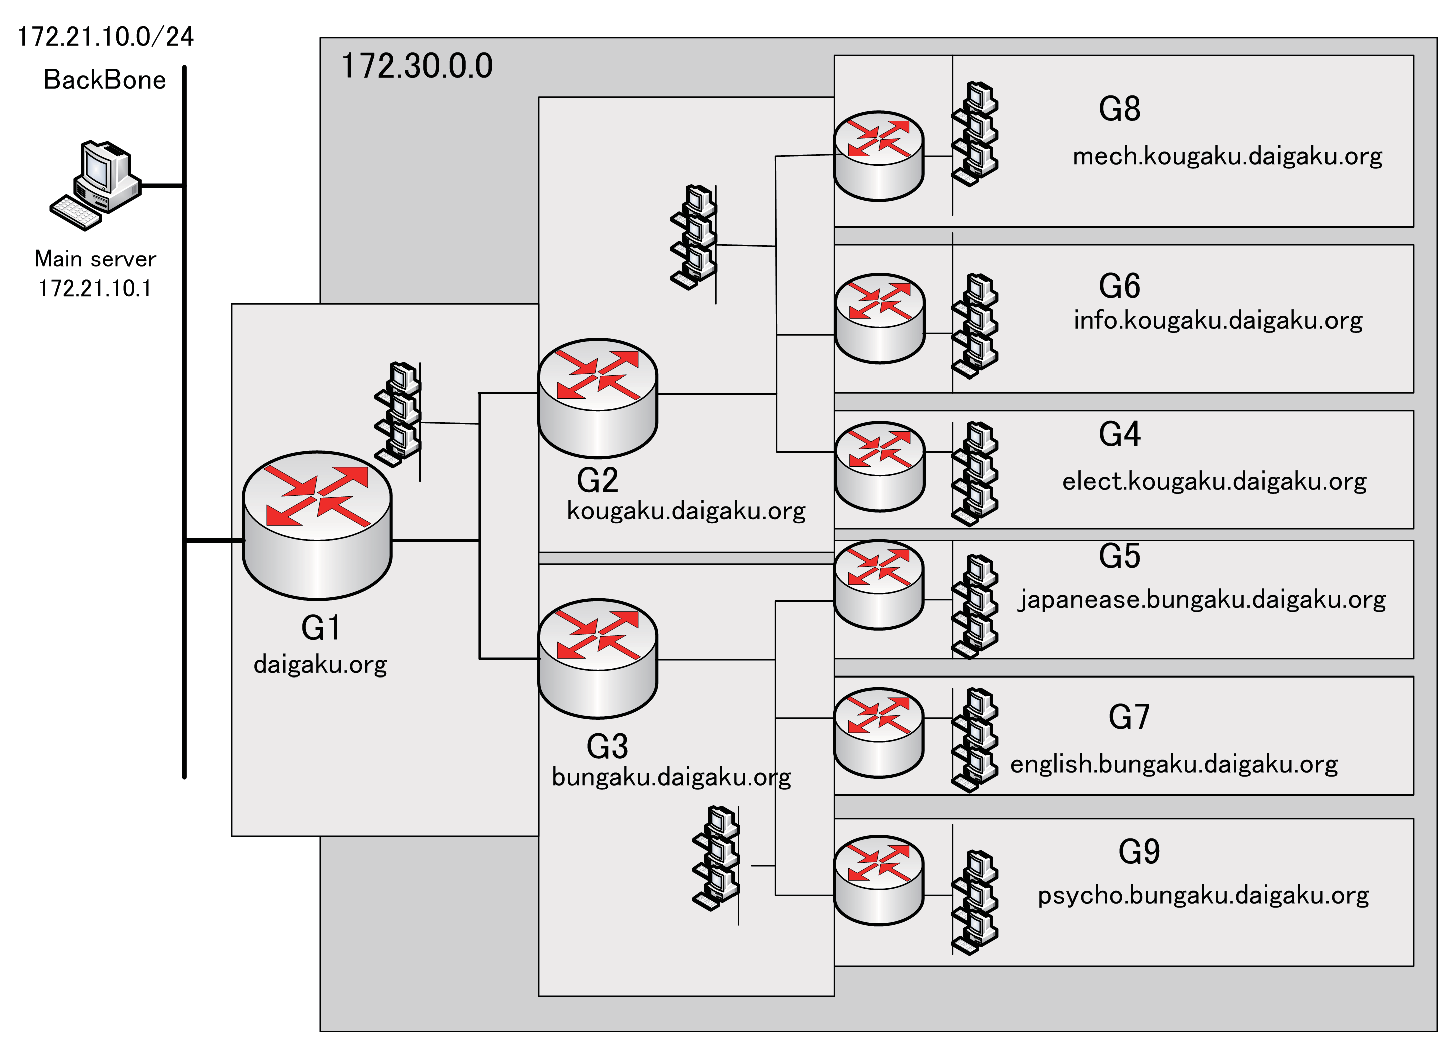
\includegraphics{./etc/specs/final.eps}}
\vspace*{-1zh}
\end{center}
\caption{最終課題構成図}
\label{final:fig:finalnet}
\end{figure}
ただし,ここで使用しているグループやドメインは仮のものであり,どのグルー
プがどこを担当し,どのようなドメイン・サブドメインにするかは後ほど決定
する.

\subsection{要求仕様}

\subsubsection{各グループのIPアドレスの割り当て}
G1以下の全体のネットワークに 172.30.0.0(ナチュラルマスク)のネットワー
クが割り当てられているので,各グループ同士で協議の上,サブネット化をし
て用いる.

\subsubsection{各グループの責任範囲}
各グループが責任を持って設定しなければならない範囲は,各グループのルー
タの上流側インターフェイスの接続・設定から下流側のサブネットワークの全
ての機器(スイッチングハブ,サーバ,コンピュータ,周辺機器,ケーブル)
である.ただし下流側ルータのインターフェイス接続は,下流側グループの担
当となる.

\subsubsection{各グループのルータのIPアドレス}
\begin{itemize}
\item 各サブネットの最も小さい IP アドレスから付与する.
\item サブネット内に複数のルータがある場合は,グループ番号の小さいものから順に付与する.
\end{itemize}

\subsubsection{ルーティング}
\begin{itemize}
\item 静的ルーティングを用いる.
\item 各ワークステーション,コンピュータ等は,デフォルトゲートウェイとして自
グループの上位側ルータを指定する.
\end{itemize}

\subsubsection{DNS ドメインの構成}
\begin{itemize}
\item G1 以下の全体ネットワークに daigaku.org ドメインが付与されている.
\item G1 が daigaku.org ゾーンを管理し,G2,G3 にそれぞれサブドメイン
  kougaku, bungaku を割り当てて,それらのゾーンを委譲する.
\item G2 は kougaku.daigaku.org ゾーンを管理し,G4,G6,G8 にそれぞれ
  elect,info,mech サブドメインを割り当て,ゾーンを委譲をする.
\item G3 は bungaku.daigaku.org ゾーンを管理し,G5,G7,G9 にそれぞれ
  japanese,english,psycho サブドメインを割り当て,ゾーンを委譲をする.
\item G4 は elect.kougaku.daigaku.org ゾーンを管理する.
\item G5 は japanese.bungaku.daigaku.org ゾーンを管理する.
\item G6 は info.kougaku.daigaku.org ゾーンを管理する.
\item G7 は english.bungaku.daigaku.org ゾーンを管理する.
\item G8 は mech.kougaku.daigaku.org ゾーンを管理する.
\item G9 は psycho.bungaku.daigaku.org ゾーンを管理する.
\item 逆引きは考えなくてよい(設定を行う必要はない).
\end{itemize}

\subsubsection{外部ネットワークとの接続}
\begin{itemize}
\item 各グループのサーバ間は,接続可能であること.
\item 各グループのサーバは,Mail server 172.21.10.1 に接続可能であること.
\item 各グループのサーバは,backbone 172.21.10.0/24 に接続可能であること.
\end{itemize}

\subsubsection{サービス}
\begin{itemize}
\item 全ての端末からメール送受信,ウェブ閲覧が行えること.
\item メールアカウントは全員分作成する.
\item その他,必要と感じるサービス,便利であると考えるサービスがあれば
  構築する.構築したサービスについては,レポートに記述すること.
\end{itemize}


\subsubsection*{考慮すべき点}
\begin{itemize}
\item どのようにネットワークの設計を行うか
\item どのような設定をして要求する仕様を満たすか.
\item ネットワークのポリシーはどのように設定すべきか.
\item 他者との共同作業をどのように行うべきか.
\item どこまでが自分の責任範囲で,どこからが他者に責任範囲か.
\item 他者への設定依頼はどのようにすべきか.
\end{itemize}


\clearpage


%------------------------------------------------------------------- 参考文献
%\input{reference.tex}

\end{document}
